\documentclass[DM,lsstdraft,toc]{lsstdoc}

\setDocChangeRecord{%
\addtohist{1.1}{2004-06-23}{Initial version (Document-139).}{J.~Kantor}
\addtohist{1.2}{2011-07-12}{Updated for PDR.}{J.~Kantor}
\addtohist{1.3}{2014-03-07}{Updated for construction phase.}{J.~Kantor}
\addtohist{1.4}{2014-10-21}{SQuaRE section added.}{J.~Kantor}
\addtohist{1.5}{2014-10-30}{Added LDM-294 handle.}{J.~Kantor}
\addtohist{2.0}{2015-03-11}{Updated with new RFC process, realignment of TCT, SAT, DMLT.}{J.~Kantor}
\addtohist{3.0}{2017-06-30}{Complete overhaul of content, with all new authors. Rewritten in LaTeX. Approved for release by W.~O'Mullane.}{W.~O'Mullane}
\addtohist{3.1}{2017-07-04}{Minor cleanups for review. Approved in \jira{RFC-358}.}{W.~O'Mullane}
\addtohist{3.2}{2017-07-19}{Editorial fixes and refresh schedule and component  diagrams}{W.~O'Mullane}
\addtohist{3.3}{2017-08-21}{Update CCB and SE groups. Add Science Platform Scientist. Add section on design reviews. Approved in \jira{RFC-373}.}{W.~O'Mullane}
\addtohist{3.4}{2017-12-21}{Org chart refresh - rules for review of epics \jira{DM-7501}}{W.~O'Mullane}
\addtohist{3.5}{2018-06-18}{New DM product tree and revised org chart. Add deputy subsystem scientist. Approved in \jira{RFC-493}}{J.~Swinbank}
\addtohist{3.6}{2019-01-29}{Review product tree. Add release management subsection. Update DMCCB and DMSE team. Approved in \jira{RFC-561}}{G.~Comoretto}
\addtohist{3.7}{2019-02-06}{Add text for LSP and Middleware mangers. Time allocation policy for institutional scientists, add admin names to org chart. Approved in \jira{RFC-572}}{W.~O'Mullane, L.~Guy}
\addtohist{3.8}{2019-05-16}{Add glossary - org chart update }{W.~O'Mullane, L.~Guy}
}

\title[DM PMP]{Data Management Organization and Management}

\author   {William O'Mullane, John Swinbank, Mario Juric, Leanne Guy and DMLT}
\setDocRef      {LDM-294} % the reference code
\setDocDate     {\today}              % the date of the issue
\setDocUpstreamLocation{\url{https://github.com/lsst/LDM-294}}

%
% a short abstract
%
\setDocAbstract {
This management plan covers the organization and management of the Data Management (DM) subsystem during the development, construction, and commissioning of LSST.
It sets out DM goals and lays out the management organization roles and responsibilities to achieve them.
It provides a high level overview of DM architecture, products and processes.
It provides a structured starting point for understanding DM and pointers to further documentation.}

% DO NOT EDIT - generated by /Users/womullan/LSSTgit/lsst-texmf/bin/generateAcronyms.py from https://lsst-texmf.lsst.io/.
\newglossaryentry{2D} {name={2D}, description={Two-dimensional}}
\newacronym{AP} {AP} {Alert Production}
\newacronym{API} {API} {Application Programming Interface}
\newglossaryentry{AURA} {name={AURA}, description={\gls{Association of Universities for Research in Astronomy}}}
\newglossaryentry{Alert} {name={Alert}, description={A packet of information for each source detected with signal-to-noise ratio > 5 in a difference image during Prompt Processing, containing measurement and characterization parameters based on the past 12 months of LSST observations plus small cutouts of the single-visit, template, and difference images, distributed via the internet.}}
\newglossaryentry{Alert Production} {name={Alert Production}, description={The principal component of Prompt Processing that processes and calibrates incoming images, performs Difference Image Analysis to identify DIASources and DIAObjects, packages and distributes the resulting Alerts, and runs the Moving Object Processing System.}}
\newglossaryentry{Archive} {name={Archive}, description={The repository for documents required by the NSF to be kept. These include documents related to design and development, construction, integration, test, and operations of the LSST observatory system. The archive is maintained using the enterprise content management system DocuShare, which is accessible through a link on the project website www.project.lsst.org.}}
\newglossaryentry{Archive Center} {name={Archive Center}, description={Part of the LSST Data Management System, the LSST archive center is a data center at NCSA that hosts the LSST Archive, which includes released science data and metadata, observatory and engineering data, and supporting software such as the LSST Software Stack.}}
\newglossaryentry{Association Pipeline} {name={Association Pipeline}, description={An application that matches detected Sources or DIASources or generated Objects to an existing catalog of Objects, producing a (possibly many-to-many) set of associations and a list of unassociated inputs. Association Pipelines are used in Prompt Processing after DIASource generation and in the final stages of Data Release processing to ensure continuity of Object identifiers.}}
\newglossaryentry{Association of Universities for Research in Astronomy} {name={Association of Universities for Research in Astronomy}, description={ consortium of US institutions and international affiliates that operates world-class astronomical observatories, AURA is the legal entity responsible for managing what it calls independent operating Centers, including LSST, under respective cooperative agreements with the National Science Foundation. AURA assumes fiducial responsibility for the funds provided through those cooperative agreements. AURA also is the legal owner of the AURA Observatory properties in Chile.}}
\newglossaryentry{Base Facility} {name={Base Facility}, description={The data center located at the Base Site in La Serena, Chile. The Base Facility is composed of the Base portion of the Prompt Enclave directly supporting Observatory operations, the Commissioning Cluster, an Archive Enclave holding data products, and the Chilean Data Access Center.}}
\newglossaryentry{Batch Production} {name={Batch Production}, description={Computational processing that is executed as inputs become available, in a distributed way across multiple enclaves when needed, while tracking status and outputs. Examples of Batch Production include offline processing for Prompt data products, calibration products, template images, and Special Programs data products. Prioritization protocols for the various types of batch production are given in LDM-148.}}
\newglossaryentry{Butler} {name={Butler}, description={A middleware component for persisting and retrieving image datasets (raw or processed), calibration reference data, and catalogs.}}
\newacronym{CC} {CC} {Change Control}
\newacronym{CCB} {CCB} {\gls{Change Control Board}}
\newglossaryentry{CCD} {name={CCD}, description={\gls{Charge-Coupled Device}}}
\newacronym{CI} {CI} {Continuous Integration}
\newglossaryentry{CMDB} {name={CMDB}, description={Configuration Management Database}}
\newglossaryentry{Calibration Scientist} {name={Calibration Scientist}, description={The person responsible for the system calibration plan who establishes the requirements for the constituent elements of the calibration hardware, software, and operational data. The Calibration Scientist works under the direction of the Systems Engineering group.}}
\newglossaryentry{Camera} {name={Camera}, description={The LSST subsystem responsible for the 3.2-gigapixel LSST camera, which will take more than 800 panoramic images of the sky every night. SLAC leads a consortium of Department of Energy laboratories to design and build the camera sensors, optics, electronics, cryostat, filters and filter exchange mechanism, and camera control system.}}
\newglossaryentry{Center} {name={Center}, description={An entity managed by AURA that is responsible for execution of a federally funded project}}
\newglossaryentry{Change Control} {name={Change Control}, description={The systematic approach to managing all changes to the LSST system, including technical data and policy documentation. The purpose is to ensure that no unnecessary changes are made, all changes are documented, and resources are used efficiently and appropriately.}}
\newglossaryentry{Change Control Board} {name={Change Control Board}, description={ "advisory board to the Project Manager; composed of technical and management representatives who recommend approval or disapproval of proposed changes to}}
\newglossaryentry{Charge-Coupled Device} {name={Charge-Coupled Device}, description={a particular kind of solid-state sensor for detecting optical-band photons. It is composed of a 2-D array of pixels, and one or more read-out amplifiers.}}
\newglossaryentry{Commissioning} {name={Commissioning}, description={A two-year phase at the end of the Construction project during which a technical team a) integrates the various technical components of the three subsystems; b) shows their compliance with ICDs and system-level requirements as detailed in the LSST Observatory System Specifications document (OSS, LSE-30); and c) performs science verification to show compliance with the survey performance specifications as detailed in the LSST Science Requirements Document (SRD, LPM-17).}}
\newglossaryentry{Construction} {name={Construction}, description={The period during which LSST observatory facilities, components, hardware, and software are built, tested, integrated, and commissioned. Construction follows design and development and precedes operations. The LSST construction phase is funded through the \gls{NSF} \gls{MREFC} account.}}
\newacronym{DAC} {DAC} {\gls{Data Access Center}}
\newacronym{DAX} {DAX} {Data Access Services}
\newacronym{DCR} {DCR} {Differential Chromatic Refraction}
\newacronym{DDMPM} {DDMPM} {Data Management Deputy Project Manager}
\newacronym{DIA} {DIA} {Difference Image Analysis}
\newglossaryentry{DIAObject} {name={DIAObject}, description={A DIAObject is the association of DIASources, by coordinate, that have been detected with signal-to-noise ratio greater than 5 in at least one difference image. It is distinguished from a regular Object in that its brightness varies in time, and from a SSObject in that it is stationary (non-moving).}}
\newglossaryentry{DIASource} {name={DIASource}, description={A DIASource is a detection with signal-to-noise ratio greater than 5 in a difference image.}}
\newacronym{DM} {DM} {\gls{Data Management}}
\newglossaryentry{DMCCB} {name={DMCCB}, description={DM Change Control Board}}
\newglossaryentry{DMIS} {name={DMIS}, description={DM Interface Scientist}}
\newglossaryentry{DMLT} {name={DMLT}, description={DM Leadership Team}}
\newacronym{DMPM} {DMPM} {Data Management Project Manager}
\newacronym{DMS} {DMS} {Data Management Subsystem}
\newacronym{DMSR} {DMSR} {DM System Requirements; LSE-61}
\newglossaryentry{DMSS} {name={DMSS}, description={DM Subsystem Scientist}}
\newglossaryentry{DMTN} {name={DMTN}, description={DM Technical Note}}
\newacronym{DOE} {DOE} {\gls{Department of Energy}}
\newacronym{DR} {DR} {Data Release}
\newacronym{DRP} {DRP} {Data Release Production}
\newglossaryentry{Data Access Center} {name={Data Access Center}, description={Part of the LSST Data Management System, the US and Chilean DACs will provide authorized access to the released LSST data products, software such as the Science Platform, and computational resources for data analysis. The US DAC also includes a service for distributing bulk data on daily and annual (Data Release) timescales to partner institutions, collaborations, and LSST Education and Public Outreach (EPO). }}
\newglossaryentry{Data Backbone} {name={Data Backbone}, description={The software that provides for data registration, retrieval, storage, transport, replication, and provenance capabilities that are compatible with the Data Butler. It allows data products to move between Facilities, Enclaves, and DACs by managing caches of files at each endpoint, including persistence to long-term archival storage (e.g. tape).}}
\newglossaryentry{Data Management} {name={Data Management}, description={The LSST Subsystem responsible for the Data Management System (DMS), which will capture, store, catalog, and serve the LSST dataset to the scientific community and public. The DM team is responsible for the DMS architecture, applications, middleware, infrastructure, algorithms, and Observatory Network Design. DM is a distributed team working at LSST and partner institutions, with the DM Subsystem Manager located at LSST headquarters in Tucson.}}
\newglossaryentry{Data Management Subsystem} {name={Data Management Subsystem}, description={The subsystems within Data Management may contain a defined combination of hardware, a software stack, a set of running processes, and the people who manage them: they are a major component of the DM System operations. Examples include the 'Archive Operations Subsystem' and the 'Data Processing Subsystem'"."}}
\newglossaryentry{Data Management System} {name={Data Management System}, description={The computing infrastructure, middleware, and applications that process, store, and enable information extraction from the LSST dataset; the DMS will process peta-scale data volume, convert raw images into a faithful representation of the universe, and archive the results in a useful form. The infrastructure layer consists of the computing, storage, networking hardware, and system software. The middleware layer handles distributed processing, data access, user interface, and system operations services. The applications layer includes the data pipelines and the science data archives' products and services.}}
\newglossaryentry{Data Release} {name={Data Release}, description={The approximately annual reprocessing of all LSST data, and the installation of the resulting data products in the LSST Data Access Centers, which marks the start of the two-year proprietary period.}}
\newglossaryentry{Data Release Production} {name={Data Release Production}, description={An episode of (re)processing all of the accumulated LSST images, during which all output DR data products are generated. These episodes are planned to occur annually during the LSST survey, and the processing will be executed at the Archive Center. This includes Difference Imaging Analysis, generating deep Coadd Images, Source detection and association, creating Object and Solar System Object catalogs, and related metadata.}}
\newglossaryentry{Department of Energy} {name={Department of Energy}, description={cabinet department of the United States federal government; the DOE has assumed technical and financial responsibility for providing the LSST camera. The DOE's responsibilities are executed by a collaboration led by SLAC National Accelerator Laboratory.}}
\newglossaryentry{Difference Image} {name={Difference Image}, description={Refers to the result formed from the pixel-by-pixel difference of two images of the sky, after warping to the same pixel grid, scaling to the same photometric response, matching to the same PSF shape, and applying a correction for Differential Chromatic Refraction. The pixels in a difference thus formed should be zero (apart from noise) except for sources that are new, or have changed in brightness or position. In the LSST context, the difference is generally taken between a visit image and template. }}
\newglossaryentry{Difference Image Analysis} {name={Difference Image Analysis}, description={The detection and characterization of sources in the Difference Image that are above a configurable threshold, done as part of Alert Generation Pipeline.}}
\newglossaryentry{Differential Chromatic Refraction} {name={Differential Chromatic Refraction}, description={The refraction of incident light by Earth's atmosphere causes the apparent position of objects to be shifted, and the size of this shift depends on both the wavelength of the source and its airmass at the time of observation. DCR corrections are done as a part of DIA.}}
\newglossaryentry{Director} {name={Director}, description={The person responsible for the overall conduct of the project; the LSST director is charged with ensuring that both the scientific goals and management constraints on the project are met. S/he is the principal public spokesperson for the project in all matters and represents the project to the scientific community, AURA, the member institutions of LSSTC, and the funding agencies.}}
\newglossaryentry{DocuShare} {name={DocuShare}, description={The trade name for the enterprise management software used by LSST to archive and manage documents}}
\newglossaryentry{Document} {name={Document}, description={Any object (in any application supported by DocuShare or design archives such as PDMWorks or GIT) that supports project management or records milestones and deliverables of the LSST Project}}
\newacronym{EFD} {EFD} {Engineering Facilities Database}
\newglossaryentry{EPO} {name={EPO}, description={Education and Public Outreach}}
\newglossaryentry{Earned Value} {name={Earned Value}, description={A measurement of how much work has been completed compared to how much was expected to have been completed at a given point in the project}}
\newglossaryentry{Enclave} {name={Enclave}, description={Individually defined portions of the computational resources at the Summit, Base, NCSA, and Satellite Facilities, such as the Prompt Enclave, the Archive Enclave, etc. }}
\newacronym{FITS} {FITS} {\gls{Flexible Image Transport System}}
\newglossaryentry{Firefly} {name={Firefly}, description={A framework of software components written by IPAC for building web-based user interfaces to astronomical archives, through which data may be searched and retrieved, and viewed as \gls{FITS} images, catalogs, and/or plots. Firefly tools will be integrated into the Science Platform.}}
\newglossaryentry{Flexible Image Transport System} {name={Flexible Image Transport System}, description={an international standard in astronomy for storing images, tables, and metadata in disk files. See the IAU FITS Standard for details.}}
\newglossaryentry{Handle} {name={Handle}, description={The unique identifier assigned to a document uploaded to DocuShare}}
\newacronym{IAU} {IAU} {International Astronomical Union}
\newglossaryentry{ICBS} {name={ICBS}, description={International Communications and Base Site}}
\newglossaryentry{IPAC} {name={IPAC}, description={No longer an acronym; science and data center at Caltech}}
\newglossaryentry{IRSA} {name={IRSA}, description={Infrared Science Archive}}
\newacronym{IT} {IT} {Integration Test}
\newacronym{ITC} {ITC} {Information Technology Center}
\newglossaryentry{IVOA} {name={IVOA}, description={International Virtual-Observatory Alliance}}
\newacronym{LDF} {LDF} {LSST Data Facility}
\newglossaryentry{LDM} {name={LDM}, description={LSST Data Management (Document Handle)}}
\newglossaryentry{LPM} {name={LPM}, description={LSST Project Management (Document Handle)}}
\newglossaryentry{LSE} {name={LSE}, description={LSST Systems Engineering (Document Handle)}}
\newglossaryentry{LSR} {name={LSR}, description={LSST System Requirements; LSE-29}}
\newacronym{LSST} {LSST} {Large Synoptic Survey Telescope}
\newglossaryentry{LSSTC} {name={LSSTC}, description={\gls{LSST} Corporation. an Arizona 501(c)3 not-for-profit corporation formed in 2003 for the purpose of designing, constructing, and operating the LSST System. During design and development, the Corporation stewarded private funding used for such essential contributions as early site preparation, mirror construction, and early data management system development. During construction, LSSTC will secure private operations funding from international affiliates and play a key role in preparing the scientific community to use the LSST dataset.}}
\newglossaryentry{LaTeX} {name={LaTeX}, description={(Leslie) Lamport TeX (document markup language and document preparation system)}}
\newacronym{MOPS} {MOPS} {Moving Object Processing System}
\newglossaryentry{MREFC} {name={MREFC}, description={\gls{Major Research Equipment and Facility Construction}}}
\newglossaryentry{Major Research Equipment and Facility Construction} {name={Major Research Equipment and Facility Construction}, description={the NSF account through which large facilities construction projects such as LSST are funded}}
\newglossaryentry{Moving Object Processing System} {name={Moving Object Processing System}, description={The Moving Object Processing System (MOPS) identifies new SSObjects using unassociated DIASources. MOPS is part of the Science Pipelines.}}
\newglossaryentry{NASA} {name={NASA}, description={National Aeronautics and Space Administration}}
\newglossaryentry{NCSA} {name={NCSA}, description={National Center for Supercomputing Applications}}
\newacronym{NET} {NET} {Network Engineering Team}
\newacronym{NSF} {NSF} {\gls{National Science Foundation}}
\newglossaryentry{National Science Foundation} {name={National Science Foundation}, description={primary federal agency supporting research in all fields of fundamental science and engineering; NSF selects and funds projects through competitive, merit-based review}}
\newacronym{OCS} {OCS} {Observatory Control System}
\newglossaryentry{OSS} {name={OSS}, description={Observatory System Specifications; LSE-30}}
\newglossaryentry{Object} {name={Object}, description={In LSST nomenclature this refers to an astronomical object, such as a star, galaxy, or other physical entity. E.g., comets, asteroids are also Objects but typically called a Moving Object or a Solar System Object (SSObject). One of the DRP data products is a table of Objects detected by LSST which can be static, or change brightness or position with time.}}
\newglossaryentry{Operations} {name={Operations}, description={The 10-year period following construction and commissioning during which the LSST Observatory conducts its survey}}
\newacronym{PDF} {PDF} {Portable Document Format}
\newacronym{PM} {PM} {Project Manager}
\newacronym{PMCS} {PMCS} {\gls{Project Management Controls System}}
\newacronym{PSF} {PSF} {Point Spread Function}
\newacronym{PST} {PST} {\gls{Project Science Team}}
\newglossaryentry{Project Management Controls System} {name={Project Management Controls System}, description={suite of tools used to organize and manage a project, including cost and schedule databases, a qualified accounting system, and change control}}
\newglossaryentry{Project Manager} {name={Project Manager}, description={The person responsible for exercising leadership and oversight over the entire LSST project; he or she controls schedule, budget, and all contingency funds}}
\newglossaryentry{Project Science Team} {name={Project Science Team}, description={an operational unit within LSST that carries out specific scientific performance investigations as prioritized by the Director, the Project Manager, and the Project Scientist. Its membership includes key scientists on the Project who provide specific necessary expertise. The Project Science Team provides required scientific input on critical technical decisions as the project construction proceeds}}
\newglossaryentry{Project Scientist} {name={Project Scientist}, description={The principal scientific advisor  to the LSST Project Manager to ensure that LSST system specifications are appropriate for achieving the scientific goals of the project; the Project Scientist also works closely with the Systems Engineering group and chairs the LSST Science Council}}
\newglossaryentry{Prompt Processing} {name={Prompt Processing}, description={The processing that occurs at the Archive Center on the nightly stream of raw images coming from the telescope, including Difference Imaging Analysis, Alert Production, and the Moving Object Processing System. This processing generates Prompt Data Products.}}
\newacronym{QA} {QA} {Quality Assurance}
\newacronym{QC} {QC} {Quality Control}
\newglossaryentry{Quality Assurance} {name={Quality Assurance}, description={All activities, deliverables, services, documents, procedures or artifacts which are designed to ensure the quality of DM deliverables. This may include \gls{QC} systems, in so far as they are covered in the charge described in LDM-622. Note that contrasts with the LDM-522 definition of “QA” as “Quality Analysis”, a manual process which occurs only during commissioning and operations. See also: Quality Control.}}
\newglossaryentry{Quality Control} {name={Quality Control}, description={Services and processes which are aimed at measuring and monitoring a system to verify and characterize its performance (as in LDM-522). Quality Control systems run autonomously, only notifying people when an anomaly has been detected. See also Quality Assurance.}}
\newacronym{RA} {RA} {Right Ascension}
\newglossaryentry{REUNA} {name={REUNA}, description={Red Universitaria Nacional}}
\newacronym{RFC} {RFC} {Request For Comment}
\newacronym{RM} {RM} {Release Manager}
\newglossaryentry{Release} {name={Release}, description={With regard to data pipelines or data products, a version that is cleared for distribution (i.e., has met QA specifications), is assigned a version identifier (e.g., 2.1), and does not evolve in the future to enable provenance.}}
\newglossaryentry{Review Hub} {name={Review Hub}, description={An LSST website that acts as a clearinghouse for information about external reviews of all LSST components planned to occur in the next six months. The site links to review-specific websites for both planned reviews and reviews that have been conducted already.}}
\newglossaryentry{Risk} {name={Risk}, description={The degree of exposure to an event that might happen to the detriment of a program, project, or other activity. It is described by a combination of the probability that the risk event will occur and the consequence of the extent of loss from the occurrence, or impact. Risk is an inherent part of all activities, whether the activity is simple and small, or large and complex.}}
\newglossaryentry{Risk Management} {name={Risk Management}, description={The art and science of planning, assessing, and handling future events to avoid unfavorable impacts on project cost, schedule, or performance to the extent possible. Risk management is a structured, formal, and disciplined activity focused on the necessary steps and planning actions to determine and control risks to an acceptable level. Risk Management is an event-based management approach to managing uncertainty.}}
\newacronym{SEM} {SEM} {\gls{Systems Engineering Manager}}
\newglossaryentry{SLAC} {name={SLAC}, description={No longer an acronym; formerly Stanford Linear Accelerator Center}}
\newglossaryentry{SQuaRE} {name={SQuaRE}, description={Science Quality and Reliability Engineering}}
\newglossaryentry{SRD} {name={SRD}, description={LSST Science Requirements; LPM-17}}
\newglossaryentry{SUIT} {name={SUIT}, description={Science User Interface and Tools}}
\newglossaryentry{Science Pipelines} {name={Science Pipelines}, description={The library of software components and the algorithms and processing pipelines assembled from them that are being developed by DM to generate science-ready data products from LSST images. The Pipelines may be executed at scale as part of LSST Prompt or Data Release processing, or pieces of them may be used in a standalone mode or executed through the LSST Science Platform. The Science Pipelines are one component of the LSST Software Stack.}}
\newglossaryentry{Science Platform} {name={Science Platform}, description={A set of integrated web applications and services deployed at the LSST Data Access Centers (DACs) through which the scientific community will access, visualize, and perform next-to-the-data analysis of the LSST data products.}}
\newglossaryentry{Software Stack} {name={Software Stack}, description={Often referred to as the LSST Stack, or just The Stack, it is the collection of software written by the LSST Data Management Team to process, generate, and serve LSST images, transient alerts, and catalogs. The Stack includes the LSST Science Pipelines, as well as packages upon which the DM software depends. It is open source and publicly available.}}
\newglossaryentry{Solar System Object} {name={Solar System Object}, description={A solar system object is an astrophysical object that is identified as part of the Solar System: planets and their satellites, asteroids, comets, etc. This class of object had historically been referred to within the LSST Project as Moving Objects.}}
\newglossaryentry{Source} {name={Source}, description={A single detection of an astrophysical object in an image, the characteristics for which are stored in the Source Catalog of the DRP database. The association of Sources that are non-moving lead to Objects; the association of moving Sources leads to Solar System Objects. (Note that in non-LSST usage "source" is often used for what LSST calls an Object.)}}
\newglossaryentry{Subsystem} {name={Subsystem}, description={A set of elements comprising a system within the larger LSST system that is responsible for a key technical deliverable of the project.}}
\newglossaryentry{Subsystem Manager} {name={Subsystem Manager}, description={responsible manager for an LSST subsystem; he or she exercises authority, within prescribed limits and under scrutiny of the Project Manager, over the relevant subsystem's cost, schedule, and work plans}}
\newglossaryentry{Subsystem Scientist} {name={Subsystem Scientist}, description={The principal science advisor  to a Subsystem Manager; he or she ensures that the subsystem specifications are appropriated for achieving the project's goals}}
\newglossaryentry{Summit} {name={Summit}, description={The site on the Cerro Pachón, Chile mountaintop where the LSST observatory, support facilities, and infrastructure will be built.}}
\newglossaryentry{Summit Facility} {name={Summit Facility}, description={The main Observatory and Auxiliary Telescope buildings at the Summit Site on Cerro Pachon, Chile.}}
\newglossaryentry{Systems Engineer} {name={Systems Engineer}, description={A member of the Systems Engineering group who works closely with the Systems Engineering Manager and the Systems Scientist on the integrated LSST system's various technical issues spanning the full life cycle of the entire project}}
\newglossaryentry{Systems Engineering} {name={Systems Engineering}, description={an interdisciplinary field of engineering that focuses on how to design and manage complex engineering systems over their life cycles. Issues such as requirements engineering, reliability, logistics, coordination of different teams, testing and evaluation, maintainability and many other disciplines necessary for successful system development, design, implementation, and ultimate decommission become more difficult when dealing with large or complex projects. Systems engineering deals with work-processes, optimization methods, and risk management tools in such projects. It overlaps technical and human-centered disciplines such as industrial engineering, control engineering, software engineering, organizational studies, and project management. Systems engineering ensures that all likely aspects of a project or system are considered, and integrated into a whole.}}
\newglossaryentry{Systems Engineering Manager} {name={Systems Engineering Manager}, description={individual responsible for the oversight and coordination of the LSST systems engineering efforts as well as the management of the Systems Engineering group and work package. The SEM is also the CCB Chair and as such is responsible for the execution, technical oversight, and coordination of configuration control activities.}}
\newglossaryentry{Systems Scientist} {name={Systems Scientist}, description={A member of the Systems Engineering group and chief liaison to all project scientists; the Systems Scientist works closely with the Systems Engineering Manager and is responsible for the flow-down of science requirements. The Systems Scientist ensures that acceptance testing and commissioning address the science requirements.}}
\newglossaryentry{T/CAM} {name={T/CAM}, description={Technical/Control (or Cost) Account Manager}}
\newacronym{US} {US} {United States}
\newglossaryentry{Validation} {name={Validation}, description={A process of confirming that the delivered system will provide its desired functionality; overall, a validation process includes the evaluation, integration, and test activities carried out at the system level to ensure that the final developed system satisfies the intent and performance of that system in operations}}
\newglossaryentry{Verification} {name={Verification}, description={The process of evaluating the design, including hardware and software - to ensure the requirements have been met;  verification (of requirements) is performed by test, analysis, inspection, and/or demonstration}}
\newacronym{WBS} {WBS} {\gls{Work Breakdown Structure}}
\newacronym{WCS} {WCS} {\gls{World Coordinate System}}
\newacronym{WG} {WG} {Working Group}
\newglossaryentry{WISE} {name={WISE}, description={Wide-field Survey Explorer}}
\newglossaryentry{Work Breakdown Structure} {name={Work Breakdown Structure}, description={a tool that defines and organizes the LSST project's total work scope through the enumeration and grouping of the project's discrete work elements}}
\newglossaryentry{World Coordinate System} {name={World Coordinate System}, description={a mapping from image pixel coordinates to physical coordinates; in the case of images the mapping is to sky coordinates, generally in an equatorial (RA, Dec) system. The \gls{WCS} is expressed in FITS file extensions as a collection of header keyword=value pairs (basically, the values of parameters for a selected functional representation of the mapping) that are specified in the FITS Standard.}}
\newglossaryentry{afw} {name={afw}, description={LSST's pipeline library code and primitives including images and tables.}}
\newglossaryentry{aggregate metric} {name={aggregate metric}, description={An aggregation of multiple point metrics. For example, the overall photometric repeatability for a particular tract given given the repeatability of multiple individual stars in the tract. See also: “metric”.}}
\newglossaryentry{aggregation} {name={aggregation}, description={The process of reducing multiple input values to a single output, e.g., a metric value, computed from a collection of input values. For example, a sum or average of a metric computed over patches to produce an aggregate metric at tract level. See also: “metric”, “aggregate metric”.}}
\newglossaryentry{airmass} {name={airmass}, description={The pathlength of light from an astrophysical source through the Earth's atmosphere. It is given approximately by sec z, where z is the angular distance from the zenith (the point directly overhead, where airmass = 1.0) to the source.}}
\newglossaryentry{astronomical object} {name={astronomical object}, description={A star, galaxy, asteroid, or other physical object of astronomical interest. Beware: in non-LSST usage, these are often known as sources.}}
\newglossaryentry{background} {name={background}, description={In an image, the background consists of contributions from the sky (e.g., clouds or scattered moonlight), and from the telescope and camera optics, which must be distinguished from the astrophysical background. The sky and instrumental backgrounds are characterized and removed by the LSST processing software using a low-order spatial function whose coefficients are recorded in the image metadata.}}
\newglossaryentry{calibration} {name={calibration}, description={The process of translating signals produced by a measuring instrument such as a telescope and camera into physical units such as flux, which are used for scientific analysis. Calibration removes most of the contributions to the signal from environmental and instrumental factors, such that only the astronomical component remains.}}
\newglossaryentry{camera} {name={camera}, description={An imaging device mounted at a telescope focal plane, composed of optics, a shutter, a set of filters, and one or more sensors arranged in a focal plane array.}}
\newglossaryentry{configuration} {name={configuration}, description={A task-specific set of configuration parameters, also called a 'config'. The config is read-only; once a task is constructed, the same configuration will be used to process all data. This makes the data processing more predictable: it does not depend on the order in which items of data are processed. This is distinct from arguments or options, which are allowed to vary from one task invocation to the next.}}
\newglossaryentry{flux} {name={flux}, description={Shorthand for radiative flux, it is a measure of the transport of radiant energy per unit area per unit time. In astronomy this is usually expressed in cgs units: erg/cm2/s.}}
\newglossaryentry{git} {name={git}, description={A distributed revision control system, often used for software source code. See the Git User Manual for details. Not developed by LSST DM.}}
\newglossaryentry{metadata} {name={metadata}, description={General term for data about data, e.g., attributes of astronomical objects (e.g. images, sources, astroObjects, etc.) that are characteristics of the objects themselves, and facilitate the organization, preservation, and query of data sets. (E.g., a FITS header contains metadata).}}
\newglossaryentry{metric} {name={metric}, description={A measurable quantity which may be tracked. A metric has a name, description, unit, references, and tags (which are used for grouping). A metric is a scalar by definition. See also: aggregate metric, model metric, point metric.}}
\newglossaryentry{metric value} {name={metric value}, description={The result of computing a particular metric on some given data. Note that metric values are typically computed rather than measured. See also: metric.}}
\newglossaryentry{model metric} {name={model metric}, description={A metric describing a model related to the data. For example, the coefficients of a 2D polynomial fit to the background of a single CCD exposure.}}
\newglossaryentry{monitoring} {name={monitoring}, description={In DM QA, this refers to the process of collecting, storing, aggregating and visualizing metrics.}}
\newglossaryentry{patch} {name={patch}, description={An quadrilateral sub-region of a sky tract, with a size in pixels chosen to fit easily into memory on desktop computers.}}
\newglossaryentry{pipeline} {name={pipeline}, description={A configured sequence of software tasks (Stages) to process data and generate data products. Example: Association Pipeline.}}
\newglossaryentry{point metric} {name={point metric}, description={A metric that is associated with a single entry in a catalog. Examples include the shape of a source, the standard deviation of the flux of an object detected on a Coadd, the flux of an source detected on a difference image.}}
\newglossaryentry{provenance} {name={provenance}, description={Information about how LSST images, Sources, and Objects were created (e.g., versions of pipelines, algorithmic components, or templates) and how to recreate them.}}
\newglossaryentry{shape} {name={shape}, description={In reference to a Source or Object, the shape is a functional characterization of its spatial intensity distribution, and the integral of the shape is the flux. Shape characterizations are a data product in the DIASource, DIAObject, Source, and Object catalogs.}}
\newglossaryentry{sky map} {name={sky map}, description={A sky tessellation for LSST. The Stack includes software to define a geometric mapping from the representation of World Coordinates in input images to the LSST sky map. This tessellation is comprised of individual tracts which are, in turn, comprised of patches.}}
\newglossaryentry{stack} {name={stack}, description={A record of all versions of a document uploaded to a particular DocuShare handle}}
\newglossaryentry{tract} {name={tract}, description={A portion of sky, a spherical convex polygon, within the LSST all-sky tessellation (sky map). Each tract is subdivided into sky patches.}}
\newglossaryentry{transient} {name={transient}, description={A transient source is one that has been detected on a difference image, but has not been associated with either an astronomical object or a solar system body.}}

\makenoidxglossaries
\begin{document}
%
% the title page
%
\maketitle

%
% It's all yours from here on
%
\section{Introduction}
\subsection{Purpose}
This document defines the mission, goals and objectives, organization and responsibilities of the LSST Data Management (DM).  The document is currently scoped to define these elements for the LSST Design and Development, Construction, and Commissioning phases.  It does not address any ongoing mission for the DM during LSST operations.

\subsection{Mission statement}
Stand up operable, maintainable, quality services to deliver high-quality LSST data products for science and education, all on time and within reasonable cost.

\subsection{Goals And Objectives}
LSST Data Management will:
\begin{itemize}
\item Define the data products, data access mechanisms, and data management and curation requirements for the LSST
\item Assess current and LSST-time frame technologies for use in providing engineered solutions to the requirements
\item Define a secure computing, communications, and storage infrastructure and services architecture underlying LSST data management
\item Select, implement, construct, test, document, and deploy the LSST data management infrastructure, middleware, applications, and external interfaces
\item Adopt appropriate cybersecurity measures throughout data management and especially on external facing services.
\item Document the operational procedures associated with using and maintaining the LSST data management capabilities
\item Evaluate, select, recruit, hire/contract and direct permanent staff, contract, and in-kind resources in LSST and from partner organizations participating in LSST Data Management initiatives.

\end{itemize}


The DM goals in selecting and, where necessary, developing LSST software solutions are:

\begin{itemize}
	\item Acquire and/or develop solutions: To achieve its mission, LSST DM subsystem prefers to acquire and configure existing, off-the-shelf, solutions. Where no satisfactory off-the-shelf solutions are available, DM develops the software and hardware systems necessary to:
\begin{itemize}
	\item Enable the generation of LSST data products at the LSST Archive and Satellite processing center, and
	\item Enable the the serving of LSST data products from the two LSST DACs (one in the U.S., and one in Chile).
\end{itemize}
	\item Maintain coherent architecture: DM software architecture is actively managed at the subsystem level. A well engineered, and cleanly designed codebase is less buggy, more maintainable, and makes developers who work on it more productive. Where there is no significant impact on capabilities, budget, or schedule, LSST DM prefers to acquire and/or develop reusable, open source, solutions.
	\item Support reproducibility and insight into algorithms: Other than when prohibited by licensing, security, or other similar considerations, DM makes all newly developed source code public, especially the Science Pipelines code. Our primary goal in publicizing the code is to simplify reproducibility of LSST data products, and provide insight into algorithms used. The software is to be documented to achieve those goals. 
	\item Opportunities beyond LSST: LSST DM codes may be of interest and (re)used beyond the LSST project (e.g., by other survey projects, or individual LSST end-users). While enabling or supporting such applications goes beyond LSST’s construction requirements, cost and schedule-neutral technical and programmatic options that do not preclude them and allow for future generalization should be strongly preferred.


\end{itemize}

Background decision material on choices made in DM will be documented in technical notes (DMTN) which will be lodged in DocuShare (see \secref{sect:docman}).

\section{Data Management Conceptual Architecture \label{sect:dmarc}}

The \gls{DM} \gls{Subsystem} Architecture is detailed in \citeds{LDM-148}.
A few of the higher level diagrams are reproduced here to orient the reader within \gls{DM}.

During \gls{Operations}, components of the \gls{DM} \gls{Subsystem} will be installed and run in
multiple locations. These include:

\begin{itemize}
\item The \gls{Commissioning} Cluster in the \gls{Base Facility} in La Serena, Chile
\item The \gls{USDF} at \gls{SLAC} in Menlo Park
\item The \gls{IDF} running on Google
\item The \gls{US} \gls{DAC},  at \gls{SLAC} in Menlo Park
\item The Chilean \gls{DAC} in the \gls{Base Facility}
\item The \gls{FrDF} at \gls{CC-IN2P3} in Lyon, France
\item The \gls{UKDF} at \gls{ROE} in Scotland
\end{itemize}

\figref{fig:dmsdeploy} shows the various \gls{DM} components which will be used in operations and the physical compute environments in which they will be deployed.
Bulk data storage and transport between components is provided by the \gls{Data Backbone}. This complex piece of infrastructure is displayed in \figref{fig:databb}.

Science users will access the data products produced by \VRO~ through the
Science Platform, as shown in \figref{fig:sciplat}.

\figref{fig:dcs} shows the common infrastructure and services layer which underlies the compute environments.
This does not list specific technologies for management/monitoring, provisioning/deployment, or workload/workflow --- these are still being selected --- but under consideration are industry-standard tools such as Nagios, Puppet/vSphere/OpenStack/Kubernetes, and Pegasus.

\begin{figure}[htbp]
\begin{center}
\includegraphics[width=1.0\textwidth, trim={0cm 4.5cm 0cm 0cm}]{images/DMSDeployment}
\caption{DM components as deployed during \gls{Operations}. Refer to \citeds{LDM-148} for details of each component.}
\label{fig:dmsdeploy}
\end{center}
\end{figure}

\begin{figure}[htbp]
\begin{center}
\includegraphics[width=0.9\textwidth]{images/fig-rubin-science-platform}
\caption{The sub-components of the \gls{Science Platform}. \label{fig:sciplat}}
\end{center}
\end{figure}


\begin{figure}[htbp]
\begin{center}
\includegraphics[width=0.6\textwidth]{images/DataBackbone}
\caption{The \gls{Data Backbone} links all the physical components of \gls{DM}. \label{fig:databb}}
\end{center}
\end{figure}

\begin{figure}[htbp]
\begin{center}
 \includegraphics[width=\textwidth, trim={0cm 14cm 0cm 0cm}]{images/DMSCommonServices}
\caption{Common infrastructure services available at \gls{DM} locations. \label{fig:dcs}}
\end{center}
\end{figure}



\subsection{External Interfaces \& Auxiliary Data}
The \gls{DM} external interfaces are controlled by the ICDs listed in \tabref{tab:icds}.

\begin{table}
    \begin{center}
      \caption{DM Interface Control Documents \label{tab:icds}}
      \begin{tabular}{l p{0.7\textwidth}}
          \hline
          \citeds{LSE-68} & Data Acquisition Interface between \gls{Data Management} and \gls{Camera}\\
          \citeds{LSE-69} & Interface between the \gls{Camera} and \gls{Data Management}   \\
          \citeds{LSE-72} & \gls{OCS} Command Dictionary for \gls{Data Management}\\
          \citeds{LSE-75} & Control System Interfaces between the Telescope and \gls{Data Management}\\
          \citeds{LSE-76} & Infrastructure Interfaces between \gls{Summit Facility} and \gls{Data Management}\\
          \citeds{LSE-77} & Infrastructure Interfaces between \gls{Base Facility} and \gls{Data Management}\\
          \citeds{LSE-130} & List of Data Items to be Exchanged Between the \gls{Camera} and \gls{Data Management}\\
          \citeds{LSE-131} & \gls{Data Management} Interface Requirements to Support Education and Public Outreach \\
          \citeds{LSE-140} & Auxiliary Instrumentation Interface between \gls{Data Management} and Telescope\\
          \hline
      \end{tabular}
    \end{center}
\end{table}

In addition, certain tasks in \gls{DM} rely on external catalogs and other information.
The current design requires:
\begin{itemize}
\item Gaia catalog (\gls{Release} 2) as a photometry baseline.
\end{itemize}

\section{Data Management Organization Structure}

This section defines the organization structure for the period in which the DM System is developed and commissioned, up to the start of LSST Observatory operations.

The DM Project Manager (William O'Mullane), Deputy Project Manger (John Swinbank) and DM Project Scientist (Mario Juri\'c), who are known collectively as DM Management, lead the DM Subsystem.
The Project Manager has direct responsibility for coordination with the overall LSST Project Office, the LSST Change Control Board, the LSST Corporation, and LSST partner organizations on all budgetary, schedule, and resource matters.
The Project Scientist has primary scientific and technical responsibility in the DM and responsibility for ensuring that the scientific requirements of the LSST are supported, and is a member on the LSST Project Science Team (PST).

As shown in \figref{fig:dmorg}, the organization now features  major products  each with a product owner
relating to a major element of the DM Subsystem (Level 2 Work Breakdown Structure elements).

\begin{figure}[htbp]
\begin{center}
 \includegraphics[width=\textwidth]{images/DmOrg}
\caption{DM organization with Scientists in Green. \label{fig:dmorg}}
\end{center}
\end{figure}
%figure wom


\subsection {Meetings } \label{sect:meetings}
As a diverse and distributed organization DM staff will participate in a considerable number of meetings. 
NSF and Aura have many rules on meeting attendance and LSST keep policies updated accordingly on the project travel web page  \url{https://project.lsst.org/travel/policies-procedures}. This include the travel summary report template \url{https://project.lsst.org/sites/default/files/Travel/Travel%20Summary%20Report.pdf} every traveler must fill after attending a meeting.  More details are in \citeds{Document-13760}.

A detailed debrief note or presentation may be asked of travelers to specific meetings of interest by the DMLT.


\subsection {Document Management} \label{sect:docman}

DM documents will follow the System Engineering Guidelines of LSST. PDF versions of released documents shall be put in Docushare in accordance with the Project's Document Management Plan \citedsp{LPM-51}. LPM level documents are released on agreement of the DMCCB (\secref{sect:dmccb}), uncontrolled documents such as technotes may be released when the author decides it is appropriate or they are asked to release it by the Project Manager. 

The Document Tree for DM is shown in \figref{fig:doctree}, it is not exhaustive but gives a high level orientation for the main documents in DM and how they relate to each other. Some documents shown in red are not yet written.

\begin{figure}
\begin{center}
 \includegraphics[width=0.9\textwidth]{images/DocTree}
\caption{Outline of the documentation tree for DM software relating the high level documents to each other. \label{fig:doctree}}
\end{center}
\end{figure}

\figref{fig:doctree} has one box for End User documentation, this is a major set of documentation for DM which will be web based as  described in  \citeds{LDM-493}. \figref{fig:eudoc} shows the intended web hierarchy for the end user documentation.

\begin{figure}
\begin{center}
 \includegraphics[width=1\textwidth]{images/EndUserDocs}
\caption{Outline of the web hierarchy for the DM end user documentation. \label{fig:eudoc}}
\end{center}
\end{figure}
%Figure from jsick



Service-level documentation follows the layered service architecture of the LSST Data Facility (see \figref{fig:servdoc}).

\begin{figure}
\begin{center}
 \includegraphics[width=0.5\textwidth]{images/servdocs}
\caption{Outline of layered service architecture of the Data Facility. \label{fig:servdoc}}
\end{center}
\end{figure}

\subsubsection {Documentation of Cross-Cutting Aspects for services}

The cross-cutting aspects of the LSST Data Facility, Security and Operational Manageability, are represented by the vertical boxes. Documentation of these aspects describes policies, procedures, and supporting management frameworks, including:
\begin{enumerate}
	\item	LDF service management framework: service catalog, service-level agreements (SLAs), configuration management database (CMDB), service monitoring.
	\item	LDF service management processes and context in the overall project: incident response, request response, issue tracking, problem management and the problem management database, change management and change control authority, release management.
	\item	Overview of the security enclave structure
	\item	Security controls and incident response procedures
	\item	Disaster recovery and continuity policies
\end{enumerate}

\subsubsection{Documentation of Service Layers}

The box at the top of the figure, Use Cases, represents subsystem-level and project-level operational use cases. The next layer, LDF-offered Services, represents specific services offered by the Data Facility which satisfy those use cases. Documentation of this layer includes:

\begin{enumerate}
\item	For each service, a Concept of Operations (ConOps) which summarizes how a service operates to satisfy a use case. The ConOps describes the operational characteristics of the production system, context within overall LSST operations, and representative scenarios. 
\item	For each service, a Theory of Operations, which provides a mental model of a constructed system. The Theory of Operations explains how the constructed service both fulfills the ConOps and integrates with the cross-cutting aspects of the facility. The document describes the overall architecture of the service and dependency on supporting service layers; integration into aspects of computer security, information security and business continuity; and integration into incident reporting and response, availability and capacity management, and change management.
\end{enumerate}

The next two layers, Reusable Production Services and Data, Compute, and IT Security Services, represent tiers of supporting service. Documentation of these layers includes a Theory of Operations, as described above, explaining the dependencies on supporting service and ITC layers, and integration with cross-cutting aspects of the facility.

The ITC box represents hardware components supporting all LDF services. Documentation of ITC describes the system elements at all facility sites, administration within each security enclave and integration with security operations, the overall provisioning plan, ITC system monitoring and integration into the service monitoring framework, and integration into service management processes including configuration management and change management.

The Software box represents service software components being developed by the LSST Data Facility. Documentation of software elements follows the standards of the LSST software stack.

Documents are managed as configuration items in the LSST Data Facility CMDB.

\subsubsection{Draft Documents}

Draft DM documents will be kept in GitHub. A single repository per document will be maintained with the head revision containing the {\em released } version which should match the version on docushare. Each repository will be included as a {\em submodule} of a single git repository located at \url{https://github.com/lsst-dm/dm-docs}.

Use of Google Docs or confluence is tolerated but final delivered documents must conform to the standard LSST format, and hence either produced with LaTeX, using the lsst-texmf package\footnote{\url{https://lsst-texmf.lsst.io}}, or Word, using the appropriate LSST template \citedsp{Document-9224, Document-11920}. The precursor document should then be erased with a pointer to the baseline document, stored in GitHub.

End user documentation will most likely and appropriately be web based and the scheme for that is described in \citeds{LDM-493}.

\subsection {Configuration Control} \label{sect:config}

Configuration control of documents is dealt with in \secref{sect:docman}. Here we consider more the operational systems and software configuration control.

\subsubsection{Software Configuration Control}

DM follows a git based versioning system based  on public git repositories and the approach is covered in the developer guide \url{https://developer.lsst.io/}.
The master branch is the stable code with development done in {\em ticket} branches (named with the id of the corresponding Jira Ticket describing the work.
Once reviewed a branch is merged to master.\footnote{LSE-14 seem out of date and should be updated or revoked - titled a guideline it seems inappropriate as an LSE.}

As we approach commissioning and operations DM will have a much stricter configuration control.
At this point there will be a version of the software which may need urgent patching, a next candidate release version of the software, and the master.
A patch to the operational version will require the same fix to be made in the two other versions.
The role of the DM Change Control Board (DMCCB; \secref{sect:dmccb}) becomes very important at this point to ensure only essential fixes make it to the live system as patches and that required features are included in planned releases.

We cannot escape the fact that we  will have multiple code branches to maintain in operations which will lead to an increase in work load.
Hence one should consider that perhaps more manpower may be needed in commissioning to cope with urgent software fixes while continuing development.
The other consideration would be that features to be developed post commissioning will probably be delayed more than one may think, as maintenance will take priority.\footnote{WOM identifies this as the maintenance surge.}

\subsubsection{Hardware Configuration Control}

On the hardware side we have multiple configurable items, we need to control which versions of software are on which machines. These days tooling like Puppet make this reasonably painless. Still the configuration  must be carefully controlled to ensure reproducible deployments providing correct and reproducible results. The exact set of released software and other tools on each system should be held in a configuration item list.
Changes to the configuration should be endorsed by the DMCCB.

The sizing model for compute hardware purchasing is detailed in \citeds{LDM-144} \citeds{LDM-141} and \citeds{LDM-138}.

\subsection {Risk Management } \label{sect:risk}

Risks will be dealt with within the LSST Project framework as defined in \citeds{LPM-20}.
Risks in DM may be sent to the DM project manger or Deputy project manager at any time for consideration to be included in the formal risk register (appropriate costed and weighted). All risks are reviewed regularly by the DM Project manager and System engineer (minimum each 3 months). 


\subsection {Quality Assurance  } \label{sect:pa}

In accordance with the project QA plan \citeds{LPM-55} we will perform QA on the software products.
This work will mainly be carried out by SQuaRE (\secref{sect:square}).
Quality assurance here means compliance with project guidelines for production, in out case of software production. 
A part of this is to have a verification/validation plan(s) which in and of itself is a major task (see \secref{sect:vanv}).


\subsection{Action item control}
Actions in DM are tracked as Jira issues an periodically reviewed at DMLT meetings.


\subsection {Verification and Validation } \label{sect:vanv}

We intend to verify and validate as much of DM as we can before commissioning and operations.
This will be achieved through testing and operations rehearsals/data challenges.
The verification and validation approach is detailed in \citeds{LDM-503} including a high level test schedule,
the top level schedule is given in \figref{fig:schedule}.



\newpage
\section{Project controls}\label{sect:dmpc}

DM follows the LSST project controls system, as described in \citeds{LPM-98}.
Considerations specific to DM are outlined in \secref{sect:plan}.

The DM Project Controller is responsible for the PMCS and, in particular, for ensuring that DM properly complies with our earned value management requirements.
The Controller is the first point of contact for all questions about the PMCS.

\subsection{Schedule}\label{sect:schedule}

The entire LSST project schedule is held in Primavera.
Tied to major project milestones we have a series of DM tests which need to be performed to show readiness for the different project phases.
This is depicted in \figref{fig:schedule}.

\begin{figure}[htbp]
	\begin{center}
		 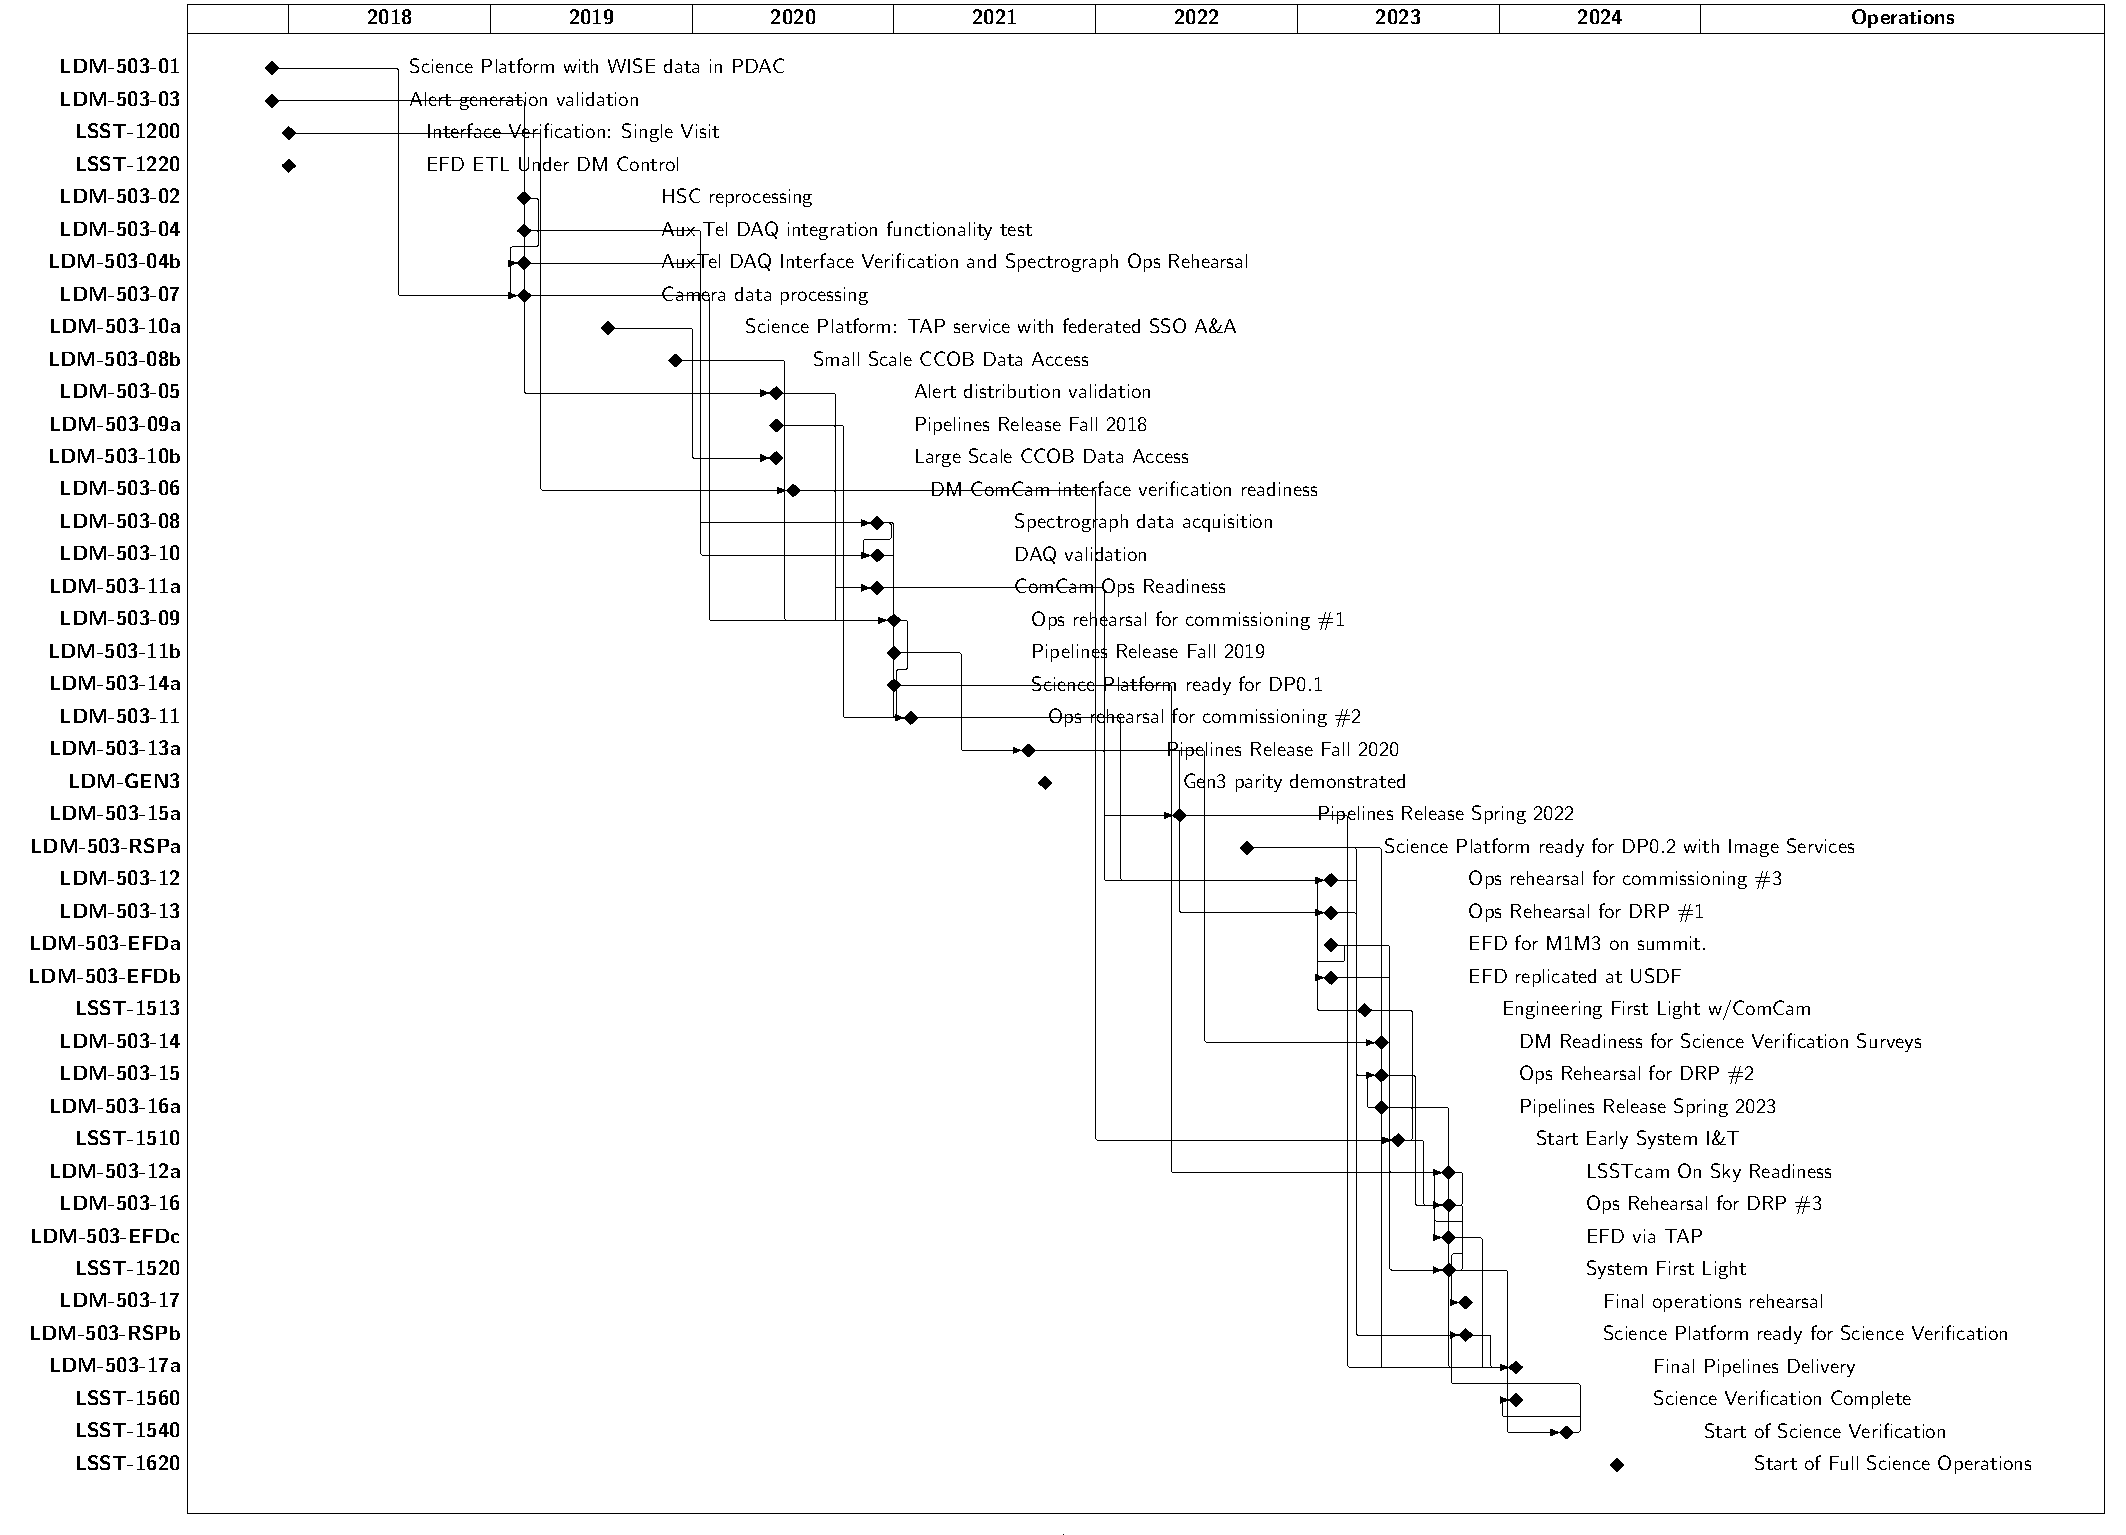
\includegraphics[width=\textwidth]{gantt}
		 \caption{DM major milestones---designated as LDM-503-\textit{x}---in
         the LSST schedule. These milestones are defined at level 2 according
         to the scheme described in \secref{sect:plan}.}
         \label{fig:schedule}
	 \end{center}
 \end{figure}

\subsection{Work breakdown structure}\label{sect:WBS}

While the original DM WBS is laid out in \citeds{LPM-43} with definitions provided in \citeds{LPM-44},
the new WBS is currently described in \appref{sec:wbslist}, which is expected to replace the contents of LPM-43 upon approval by the LSST CCB.

The WBS provides a hierarchical index of all hardware, software, services, and other deliverables which are required to complete the LSST Project.
It consists of alphanumeric strings separated by periods.
The first component is always “1”, referring to the LSST Construction Project.
``02C'' in the second component corresponds to Data Management Construction.
Subdivisions thereof are indicated by further digits.
These subdivisions correspond to teams within the DM project.
The top level WBS elements are mapped to the lead institutes in \tabref{tab:wbs}; the lead institutions roles are outlined in \secref{sect:leadtutes}.
The various groups involved in the WBS are briefly described in \secref{sect:groups}.

\begin{table}
\caption{DM top level Work Breakdown Structure \label{tab:wbs}}
\begin{center}
\begin{tabular}[htb]{|l|l|l|} \hline
\textbf{WBS}  &  \textbf{Description}   &  \textbf{Lead Institution}\\ \hline
1.02C.01& System Management                         &  LSST Tucson \\ \hline
1.02C.02& Systems Engineering                       &  LSST Tucson \\ \hline
1.02C.03& Alert Production                          &  University of Washington\\ \hline
1.02C.04& Data Release Production                   &  Princeton University\\ \hline
1.02C.05& Science User Interface and Tools          & IPAC\\ \hline
1.02C.06& Science Data Archive                      & SLAC\\ \hline
1.02C.07& LSST Data Facility                        & NCSA\\ \hline
1.02C.08& International Communications \& Base Site & LSST Tucson \\ \hline
1.02C.09& System Level Testing \& Science Validation& LSST Tucson \\ \hline
1.02C.10& Science Quality \& Reliability Engineering& LSST Tucson \\ \hline
\end{tabular}
\end{center}
\end{table}

\subsection{Planning Process}\label{sect:plan}

Milestones have been defined to describe the major goals of the DM subsystem throughout the construction project.
Each milestone has a description, a due date, and a level.
Four levels are defined:

\begin{description}
\item[Level 1]{The most important milestones exposed at the NSF level.}
\item[Level 2]{Cross-subsystem milestones (for example, DM milestones that affect the Camera Subsystem).}
\item[Level 3]{Cross-team milestones within DM (for example, Middleware milestones that affect the DRP Team).}
\item[Level 4]{Internal milestones within a team.}
\end{description}

The major DM subsystem tests described in \secref{sect:schedule} are defined as level 2 milestones.
Teams plan their work towards each test by defining a series of level 3 milestones.
Teams may define level 4 milestones for their own use.

Resources to achieve the milestones throughout the duration of construction have been allocated by means of \textit{planning packages} loaded into the PMCS.
Each top level WBS within DM (per \tabref{tab:wbs}) is divided into some tens of planning packages, each of which addresses some part of the DM baseline design with a clearly defined scope, deliverable, resource cost, and end date.

As the due date for work approaches, the actions required to complete each planning package---and hence meet the associated milestones---must be defined in detail.
The DM team divides the year into two six month long \textit{cycles}, running from November through May (the ``spring cycle'') and from June through October (the ``fall cycle'').
At the start of each cycle, the DM Leadership Team (\secref{sect:dmlt}) agrees on the detailed plan of work for the cycle, and this is loaded in to Jira as a series of ``epics'', corresponding to projects of a few person-months duration, each with defined start and end dates and resource loading.
The DM team records work and tracks progress against epics using Jira; the Project Controller (\secref{role:pcon}) arranges for this information to be ingested to and made available within the PMCS.
When epics are closed the T/CAM should ensure the deliverables are mentioned/linked in the associated comments in Jira. The DMPM shall verify all closed epics have the defined deliverables associated with them.

This process is described in detail in \citeds{DMTN-020}.

\section{Products \label{sect:products}}

The products of DM are not the data products defined in \citeds{LSE-163}, rather they are the artifacts, systems and services  we need to produce those products. \secref{sect:dmarc} outlines the highest level of this for DM while  \appref{sect:prodlist}  defines the complete product tree for DM and it is pictorially represented at a trimmed level in  \figref{fig:prods}.
\citeds{LDM-148} provides a trace of products to requirements, while \appref{sect:prodlist} proves a full list with technical manager, WBS element and product owner for each.
Our primary guiding requirements come from \citeds{LSE-30}, the Observatory System Specification (OSS), with \appref{sect:tracefor} tracing DM requirements \citedsp{LSE-61} to OSS, and \appref{sect:traceback} tracing the relevant OSS requirements to DM.

\begin{figure}[htbp]
	\begin{center}
		 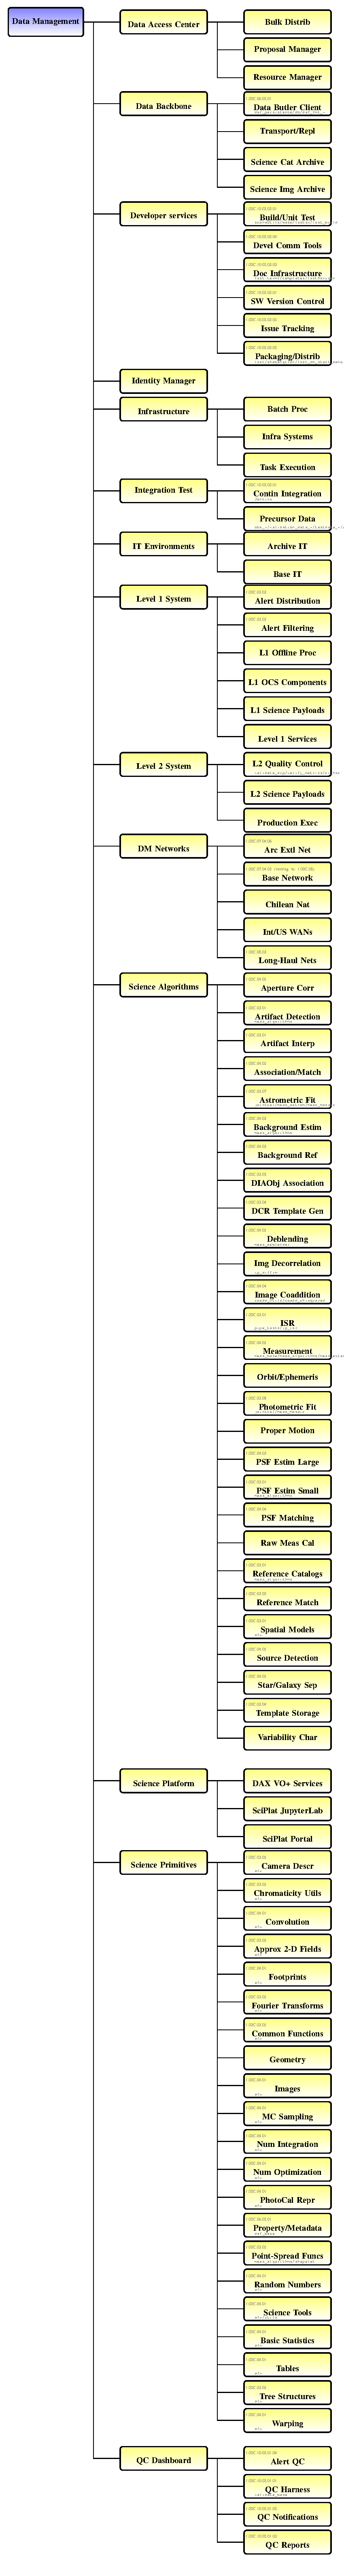
\includegraphics[height=19cm]{ProductTree}
		 \caption{DM product tree. \label{fig:prods}
		 The full list is given in \appref{sect:prodlist}
	 }

	 \end{center}
 \end{figure}

\figref{fig:prods}
 contains the WBS element associated with the component as well as any git repositories belonging to them.
 Since the figure stops at level 3 most git repositories will only be found in the full list in \appref{sect:prodlist}.

 Every git repository should appear in \appref{sect:prodlist}  and hence have a technical manager and product owner identified. The table is hierarchical hence if the manager/owner is not filled in (or the individual is no longer with the project) we may go to the parent element manager/owner. Some work remains to finish rationalizing the components and repositories.

 Every JIRA component should map to one row in \appref{sect:prodlist} thus providing a contact for that component.
 Some JIRA components are not physical products - they should still appear in the \appref{sect:prodlist} which is the single source for DM of component  ownership. Some work is also needed to rationalize the JIRA components.

\section{Roles in Data Management}

This section describes the responsibilities associated with the roles shown in
\figref{fig:dmorg}.


\subsection{DM Project Manager (DMPM)\label{role:dmpm}}

The DM Project Manager is responsible for the efficient coordination of all LSST activities and responsibilities assigned to the Data Management Subsystem. The DM Project Manager has the responsibility of establishing the organization, resources, and work assignments to provide DM solutions.  The DM Project Manager serves as the DM representative in the LSST Project Office and in that role is responsible for presenting DM initiative status and submitting new DM initiatives to be considered for approval. Ultimately, the DM Project Manager, in conjunction with his / her peer Project Managers (Telescope, Camera), is responsible for delivering an integrated LSST system. The DM Project Manager reports to the LSST Project Manager. Specific responsibilities include:

\begin{itemize}
\item Manage the overall DM System
\item Define scope and request funding for DM System
\item Develop and implement the DM project management and control process, including earned value management
\item Approve the DM Work Breakdown Structure (WBS), budgets and resource estimates
\item Approve or execute as appropriate all DM outsourcing contracts
\item Convene and/or participate in all DM reviews
\item Co-chair the DM Leadership Team (\secref{sect:dmlt})
\end{itemize}

\subsection{DM Deputy Project Manager (DDMPM) \label{role:dmdpm}}
The PM and deputy will work together on the general management of DM and any specific PM tasks may be delegated to the deputy as needed and agreed. In the absence of the PM the deputy carries full authority and decision making powers of the PM. The DM Project Manager will keep the Deputy Project Manager informed of all DM situations such that the deputy may effectively act in place of the Project Manager when absent.

\subsection{DM Subsystem Scientist (DMSS) \label{role:dmps} }

The DM Subsystem Scientist (DMSS) has the ultimate responsibility for ensuring DM initiatives provide solutions that meet the overall LSST science goals. As such, they lead the definition and understanding of the science goals and deliverables of the LSST Data Management System, and are accountable for communicating these to the DM engineering team.

The DM Subsystem Scientist reports to the LSST Project Scientist. The DMSS are a member of the LSST Change Control Board and the Project Science Team. They chair and direct the work of the DM System Science Team (\secref{sect:dmsst}).

Specific responsibilities and authorities include ({\bf cite the project-level R2A2 document, once issued}):


\begin{itemize}
\item Communicates with DM science stakeholders (LSST Project Scientist and Team, advisory bodies, the science community) to understand their needs and identifies aspects to be satisfied by the DM Subsystem.
\item Develops, maintains, and articulates the vision of DM products and services responsive to stakeholder needs.
\item Works with the LSST Project Scientist to communicate the DM System vision to DM stakeholders. Works with the DM Project Manager to communicate and articulate the DM System vision and requirements to the DM construction team.
\item Regularly monitors DM construction team progress and provides feedback to the DM Project Manager to ensure the continual understanding of and adherence to the DM vision, requirements, and priorities.
\item Develops and/or evaluates proposed changes to DM deliverables driven by schedule, budget, or other constraints.
\item Provides advice to the DM Project Manager on science-driven prioritization of construction activities. 
\item Validates the science quality of DM deliverables and the capability of all elements of the DM System to achieve LSST science goals.
\item Serves as Data Management Liaison as requested by LSST Science Collaborations
\item Provides safe, effective, efficient operations in a respectful work environment.
\end{itemize}

Specific authorities include ({\bf cite the project-level R2A2 document, once issued}):

\begin{itemize}
\item Defines the vision and high-level requirements of the DM products and services required to deliver on LSST science goals.
\item Defines the science acceptance criteria for DM deliverables (both final and intermediate) and validates that they have been met (Science Validation).
\item Hires or appoints DM System Science Team staff and other direct reports and defines their responsibilities.
\item Advises and consents to the appointments of institutional DM Science Leads.
\item Delegates authority and responsibility as appropriate to institutional Science Leads and other members of the DM System Science Team.
\item Represents and speaks for the LSST Data Management.
\item Convenes and/or participates in all DM reviews.
\item Co-Chairs the DM Leadership Team
\end{itemize}

\subsection{Project Controller/Scheduler \label{role:pcon}}

The DM Project Controller is responsible for integrating DM's agile planning process with the LSST Project Management and Control System (PMCS). Specific responsibilities include:

\begin{itemize}

  \item{Assist T/CAMs in developing the DM plan}
  \item{Synchronize the DM plan, managed as per \citeds{LDM-472}, with the LSST PMCS}
  \item{Ensure that the plan is kept up-to-date and milestones are properly tracked}
  \item{Create reports, Gantt charts and figures as requested by the DMPM}

\end{itemize}

\subsection{Product Owner \label{role:prodo}}

A product owner is responsible for the quality and acceptance of a particular product.
The product owner should sign off on the requirements to be fulfilled in every delivery and therefore also on any descopes or enhancements.
The product owner should define tests which can be run to prove a delivery meets the requirements due for that product.

\subsection{Pipeline Scientist \label{role:pipe}}

Several DM products come together to form the LSST pipeline. The Pipeline Scientist is the product owner for the overall pipeline.

The Pipeline Scientist should:

\begin{itemize}

\item Provide guidance and test criteria for the full pipeline including how QA is done on the products
\item Keep the big picture of where the codes are going in view. Predominantly the algorithms, but also the implementation and architecture (as part of the System Engineering Team \secref{sect:sysengt}).
\item Advise on how we should attack algorithmic problems, providing continuing advice to subsystem product owners as we try new things.
\item Advise on calibration issues, provide understanding of the detectors from a DM point of view
\item Advise on the overall (scientific) performance of the system, and how we'll test it.  Thinking about all the small things that we have to get right to make the overall system good.

\end{itemize}

\subsection{Systems Engineer \label{role:sysengineer}}

With the System Engineering Team (\secref{sect:sysengt}) the Systems Engineer owns the DM entries in the risk register and is generally in charge of the \textit{process} of building DM products.

As such, the Systems Engineer is responsible for managing requirements as they pertain to DM.
This includes:

\begin{itemize}
\item Update and ensure traceability of the high level design \& requirements documents: DMSR (\citeds{LSE-61}), OSS (\citeds{LSE-30}), and LSR (\citeds{LSE-29})
\item Oversee work on lower level requirements documents
\item Ensure  that the system is appropriately modeled in terms of e.g. drawings, design documentation, etc
\item Ensure  that solid verification plans and standards are established within DM
\end{itemize}

In addition, the Systems Engineer is responsible for the process to define \& maintain DM interfaces (internal and external)

\begin{itemize}
\item Define and enforce standards for internal interfaces
\item Direct the Interface Scientist's (\secref{role:dmis}) work on external ICDs
\end{itemize}

The Systems Engineer shall chair the DM Change Control Board (\secref{sect:dmccb})

\begin{itemize}
\item Organize DMCCB processes so that the change control process runs smoothly
\item Identify RFCs requiring DMCCB attention
\item Shepherd RFCs through change control
\item Call and chair DMCCB meetings, ensuring that decisions are made and recorded
\end{itemize}

Finally, the System Engineer represents DM on the LSST CCB.

\subsection{DM Interface Scientist (DMIS) \label{role:dmis}}

The DM Interface Scientist is responsible for all internal and external interfaces to the DM Subsystem. This includes ensuring that appropriate tests for those interfaces are defined. This is a responsibility delegated from the DM System engineer (\secref{role:sysengineer}).

\subsection{Software Architect \label{role:softarc}}

The Software Architect is responsible for the overall design of the DM \textit{software} system. Specific responsibilities include:

\begin{itemize}

\item{Define the overall architecture of the system and ensuring that all products integrate to form a coherent whole}
\item{Select and advocate appropriate software engineering techniques}
\item{Choose the technologies which are used within the codebase}
\item{Minimize the exposure of DM to volatile external dependencies}

\end{itemize}

The Software Architect will work closely with the Systems Engineer (\secref{role:sysengineer}) to ensure that processes are in place for tracing requirements to the codebase and providing hooks to ensure that requirement verification is possible.

\subsection{Operations Architect \label{role:opsarc}}

\textit{Margaret or Don perhaps some text here ...}

The DM Operations Architect is responsible for ensuring that all elements of the DM Subsystem, including operations teams, infrastructure, middleware, applications, and interfaces,
come together to form an operable system.

Specific responsibilities include:

\begin{itemize}
\item Set up and coordinate  operations rehearsals
\item Ensure readiness of procedures and personnel for Operations
\item Set standards for operations e.g. procedure handling and operator logging
\item Participate in stakeholder and end user coordination and approval processes and reviews
\item Serve as a member of the LSST System Engineering Team
\end{itemize}

\subsection{Configuration Manager (CM)}\label{role:cm}

%A configuration management role exists both at DM and Data Facility levels this could be the same individual
The DM Configuration Manager (CM) is responsible for Configuration Management activities inside DM and NCSA(?).
The following list is not exhaustive, but is intended as a guideline to the CM activities:

\begin{itemize}
\item Ensure that Configuration Management Plan (CMP) is correctly applied and provide appropriate reasons in case of non conformance's
\item Define  which Configuration Items are to be managed in the Configuration Item List
\item Define the Product Baseline
\item Support changes to Configuration Items within the DMCCB
\item Manage the delivery of software products
\item Maintain the Configuration Item List
\item Manage the configuration control resources used by DM
\item Maintain an awareness of the relationship between  the elements of the Product Baseline (in order for instance to be able to answer the question: ``What is the environment and which software is installed?'')
 \item Check that the Product Assurance and CMP procedures are correctly applied when Configuration Items are changed
 \item Participate in DMCCB activities
\end{itemize}

The Configuration Manager is the secretary of the CCB and works with the support of the Scientific and Technical Leaders and participates in the CCB monitoring the development and change control process.

\subsubsection{Configuration Item List}

The Configuration Item List (CIL) is the list of items that are maintained under configuration control.
CUs and DPC need to report their configuration items in the CIL with an adequate level of details.
CIL is part of the development plan but may be written in a separate document to which the development plan refers.

The Configuration Manager in charge has to identify the configuration items to include in the CIL, with the help of the technical leader and to maintain it when changes to the configuration items happen.


\subsubsection{Release management\label{sect:relMng}}

In DM usually each product will be released once per cycle.
Additional releases may be done in case of bug fixing, urgent issues, or in case that the previous one is incomplete.

Each release needs to be identified with:

\begin{itemize}
\item Configuration Item
\item Documentation:
\subitem User Manual: to be updated each major release
\subitem Requirements Specification: to be updated each major release
\subitem Test Specification: to be updated each major release
\subitem Release Note: new document each major release, updated for patch releases
\subitem Test Report: new document each major release, updated for patch releases
\item Latest Release in the \texttt{master} branch in GitHub.
\end{itemize}
This information identifies a product baseline.

%Release preparation is in charge of the DU leader and is subject to CCB approval.
The release manager is in charge of preparing the release with the technical lead for the product.
After CCB approval, the release will be delivered to NCSA.

\subsubsection{Configuration Baseline \label{sect:BSLdef}}

A Configuration Baseline (CB) represents the approved status of the project at key milestones like formal review or at the beginning of test activities.

Configuration Baselines are applicable to hardware and software, and will include the documents that describe the CIs and their status.

\subsection{Lead Institution Senior Positions}

Each Lead Institution (as defined in \secref{sect:leadtutes}; see also \tabref{tab:wbs}) has a T/CAM and Scientific or Engineering Lead, who jointly have overall responsibility for a broad area of DM work, typically a Work Breakdown Structure (WBS) Level 2 element. They are supervisors of the team at their institution, with roles broadly analogous to those of the DM Project Manager and Project Scientist.

\subsubsection{Technical/Control Account Manager (T/CAM) \label{role:tcam}}

Technical/Control Account Managers have managerial and financial responsibility
for the engineering teams within DM. Each T/CAM is responsible for a specific set of WBS elements. Their detailed responsibilities include:

\begin{itemize}

  \item{Develop, resource load, and maintain the plan for executing the DM construction project within the scope of their WBS}
  \item{Synchronize the construction schedule with development in WBS elements managed by other T/CAMs}
  \item{Maintain the budget for their WBS and ensuring that all work undertaken is charged to the correct accounts}
  \item{Work with the relevant Science Leads and Product Owners (\secref{role:prodo}) to develop the detailed plan for each cycle and sprint as required}
  \item{Work with the DM Project Controller (\secref{role:pcon}) to ensure that all plans and milestones are captured in the LSST Project Controls system}
  \item{Perform day-to-day management of staff within their WBS}
  \item{Perform the role of ``scrum-master'' during agile development}
  \item{Report activities as required, including providing input for monthly status reportsx.}

\end{itemize}

\subsubsection{Institutional Science/Engineering Lead \label{role:scilead}}

The Institutional Science/Engineering Leads serve as product owners (\secref{role:prodo}) for the major components of the DM System (Alert Production, Data Release Production, Science User Interface etc).

In addition, they provide scientific and technical expertise to their local engineering teams.

They work with the T/CAM who has managerial responsibility for their product to define the overall construction plan and the detailed cycle plans for DM.

Institutional science leads are members of the DM System Science Team (\secref{sect:dmsst}) and, as such, report to the DM Subsystem Scientist (\secref{role:dmps}).

\section{Teams within Data Management} \label{sect:groups}

Since the DM team is distributed in terms of geography and responsibility across the LSST partner and lead institutions, mechanisms are needed to ensure that the project remains on track at all times. There are five primary coordinating bodies to ensure the management, technical, and quality integrity of the DM Subsystem.

\subsection{System Science Team \label{sect:dmsst}}

Members of the DM System Science Team (SST) work together to define, maintain, and communicate to the DM Systems Engineering team a coherent vision of the LSST DM system responsive to the overall LSST Project goals, as well as scientifically validate the as-built system (\citeds{LDM-503}, Section~9.).

\begin{figure}[htbp]
\begin{center}
\includegraphics[width=0.8\textwidth]{images/DmSSTOrg}
\caption{DM System Science Team organisation.
\label{fig:sstorg}}
\end{center}
\end{figure}



\subsubsection{Organization and Goals}
\label{sect:dm-sst-org}

The System Science Team includes:
\begin{itemize}
\item \gls{DMSS} (chair)
\item DM Science Validation Scientist
\item DM Institutional Science Leads
\item DM System Science Analysts
\item DM Science Pipelines Scientist
\end{itemize}

The System Science Team has been chartered to:
\begin{itemize}
\item Support the \gls{DMSS} (as the overall DM Product Owner) in ensuring that Data Management Subsystem's initiatives provide solutions that meet the overall LSST science goals.
\item Support the Institutional Science Leads in their roles as Product Owners for elements of the DM system their respective institutions have been tasked to deliver.
\item Support the DM Science Validation Scientist, who organizes and coordinates the science validation efforts (\citeds{LDM-503}).
\item Guide the work of System Science Analysts, who generally lead and/or execute studies needed to support SST work.
\item Provide a venue for communication with the Science Pipelines Scientist, who broadly advises on topics related to the impact of science pipelines on delivered science and vice versa (\secref{role:pipe}).
\end{itemize}

The members of the System Science Team report to the \gls{DMSS} and share the following responsibilities:
\begin{itemize}
\item Communicate with the science community and internal stakeholders to understand their needs, identifying the aspects to be satisfied by the DM Subsystem.
\item Liaise with the science collaborations to understand and coordinate any concurrent science investigations relevant to the DM Subsystem.
\item Develop, maintain, and articulate the vision of DM-delivered LSST data products and services that is responsive to stakeholder needs, balanced across science areas, well motivated, and scientifically and technologically current.
\item Work with the \gls{DMPM} and DM \glspl{T/CAM} to communicate and articulate the DM System vision and requirements to the DM engineering team.
\item Identify, develop, and champion new scientific opportunities for the LSST DM System, as well as identify risks where possible.
\item Develop change proposals and/or evaluate the scientific impact of proposed changes to DM deliverables driven by schedule, budget, or other constraints.
\item Lead the Science Verification of the deliverables of the DM subsystem.
\end{itemize}

\subsubsection{Regression Monitoring of KPMs and other Metrics}

All KPMs and other regression monitoring metrics will be calculated on a regular cadence (daily if possible).
They are monitored by the SQuaRE scientist, with status periodically reported to the System Science Team (SST).
The SQuaRE scientist brings up any major regressions to the attention of the SST, along with an initial assessment of the problem.
The SST has the responsibility of monitoring the overall system for whether it meets its key performance metrics as well as understanding any significant performance regressions in performance.
The SST may recommend further actions to the \gls{DMPM} and/or \gls{DMSS}, if necessary.
These include performing additional testing, broader root cause analysis, documenting the regression, or recommendations on the priority of fixing the regression relative to presently scheduled work.

\subsubsection{Communications}

DM System Science Team communication mechanisms are described on the SST Confluence page at \url{http://ls.st/sst}. The list of current  DM liaisons to the LSST Science Collaborations and international partners is maintained  in  \url{https://www.lsstcorporation.org/science-collaborations}

\subsubsection{Time Allocation for Institutional Science Leads}

The Institutional Science Leads fulfill the role of \textit{Product Owner} for elements of the DM system that their respective institutions have been tasked to deliver; institutional T/CAMs rely on their Scientist to provide  \emph{Product Owner}  services.
In addition, as members of the DM System Science Team, they have responsibilities as described in \ref{sect:dm-sst-org}, which result in work that is more \textit{emergent} in nature.
To balance these two roles, the \gls{DMSS} is entitled to allocate up to 50\% of the Institutional Science Leads' time to Science Team work.
If any Science Team study should require a greater commitment, additional time must be negotiated and agreed with the institutional \glspl{T/CAM}s.
This arrangement is intended to ensure both a good working relationship between the T/CAMs and scientists, and that the \gls{DMSS} maintains sufficient support from the Science Team to deliver a system that meets the overall LSST science goals.

\subsection{DM Systems Engineering Team \label{sect:sysengt}}

The Systems Engineering Team is led by the DMPM (\secref{role:dmpm}) and looks after all aspects of systems engineering.
It is comprised of not only the Systems Engineer (\secref{role:sysengineer}), but also the Software Architect (\secref{role:softarc}), Operations Architect (\secref{role:opsarc}), \gls{DMSS} (\secref{role:dmps}), Pipeline Scientist (\secref{role:pipe}), Interface Scientist (\secref{role:dmis}), and the \gls{DDMPM} (\secref{role:ddmpm}).

While the product owners (\secref{role:prodo}) help DM to create products which are fit for purpose, the Systems Engineering Team must ensure we do it correctly. This group concerns itself with (sub)system wide decisions on architecture and software engineering.

The specific tasks of this group include:

\begin{itemize}
\item Formalize the product list for DM\footnote{In this sense, ``products'' are the software and systems which produce data products, rather than the data products themselves. See also \ref{sect:products}.}
\item Formalize the documentation tree for DM, defining which documents need to be produced for each product
\item Agree the process for tracing the baseline requirements verification and validation status.
\item Agree the formal versions of documents and software which form the technical baseline, individual items will go through the CCB for formal approval.  This includes upload to docushare.
\item Perform releases of software products --- including, but not limited to, the Science Pipelines --- as needed, using tooling provided by SQuaRE (\secref{sect:square}).
\item Debug unexpected build problems:
\begin{itemize}
  \item{Resolve issues related to the underlying build infrastructure directly;}
  \item{Pass off product-specific problems to the relevant product team.}
\end{itemize}
\item Maintain the build/packaging system e.g.  newinstall.sh, lsstsw, lsst\_build and EUPS.
\end{itemize}

Some of these tasks are will be delegated to individual group members.
These individuals also are the conduit to/from the rest of the DM team to raise ideas/issues with the engineering approach.

\subsubsection{Communications}

The Systems Engineering Team will only physically meet to discuss specific topics: there will not be a regular meeting of the group outside of the one to one meetings with the DM project manager for the individuals in the group.
Discussions will be held via email until in person talks are required.

\subsection{DM Leadership Team \label{sect:dmlt}}

The purpose of the DM Leadership Team (DMLT) is to assist the DMPM  establish the scope of work and resource allocation across DM and ensure overall project management integrity across DM.
The following mandate established the DMLT:

\begin{itemize}
\item Charter/purpose
	\begin{itemize}
	\item Maintain scope of work and keep within resource allocation across DM
	\item Ensure overall project management integrity across DM
	\item Ensure Earned Value management requirements are met
	\end{itemize}
\item Membership
	\begin{itemize}
	\item Co-chaired by the \gls{DMPM} (\secref{role:dmpm}) and \gls{DMSS} (\secref{role:dmps})
	\item Lead Institution Technical/Control Account Managers (T/CAMs; \secref{role:tcam})
	\item Institutional Science or Engineering Leads (\secref{role:scilead})
	\item Members of the DM Systems Engineering Team (\secref{sect:sysengt})
	\end{itemize}
\item Responsibilities
	\begin{itemize}
	\item Prepares all budgets, schedules, plans
	\item Meets every week to track progress, address issues/risks, adjust work assignments and schedules, and disseminate/discuss general PM communications
	\end{itemize}
\end{itemize}

The DM Leadership Team and the DM Systems Engineering Team (\secref{sect:sysengt}) work in synchrony.
The DMLT makes sure the requirements and architecture/design are estimated and scheduled in accordance with LSST Project required budgets and schedules.

 \subsubsection{Communications}
A mailing list\footnote{\url{lsst-dmlt@listserv.lsstcorp.org}} exists for DMLT related messages.
On Mondays the DMLT hold a brief (30 to 45 minutes) telecon. This serves to:

\begin{itemize}
\item Allow the Project manager and DM Scientist  to pass on important project level information and general guidance.
\item Raise any blocking or priority issues across DM --- this may result in calling a splinter meeting to further discuss with relevant parties.
\item Inform all team members of any change requests (LCRs) in process at LSST level which may be of interest to or have an impact on DM
\item Check on outstanding actions on DMLT members
\end{itemize}

Face to Face meetings of DM are held twice a year\footnote{One of these has been virtual since late 2018 and with COVID-19 its not obvious we will return soon to in person meetings.}; these are opportunities to:

\begin{itemize}
\item Discuss detailed planning for the next cycle
\item Discuss technical topics in a face to face environment
\item Work together on critical issues
\item Help make DM function as a team
\end{itemize}

\subsection{DM Change Control Board \label{sect:dmccb}}

The DMCCB has responsibility for issues similar to those of the LSST Change Control Board, but focused on the DM Subsystem.
The DMCCB reviews and approves changes to all baselines in the Subsystem, including proposed changes to the DM System Requirements (DMSR), reference design, sizing model, i.e. any LDM-series document.
The Technical Baseline, including software/hardware and documentation, is produced by DM and controlled by the DMCCB.
DMCCB validates that the form and content of the Technical Baseline is consistent with LSST project standards such as the Systems Engineering Management Plan (SEMP) \citeds{LSE-17}.

\begin{itemize}
\item Responsibilities:
        \begin{itemize}
        \item Determine when deliverables (controlled documents and software) are ready to be baselined (placed under configuration controlled status) or released. This include LDM series documents.
        \item Review and approve/reject proposed changes to baselined items - any LCR must go through the DMCCB before being submitted to the project CCB.
        \item Review all RFCs and approves \textit{flagged} RFCs prior to 'Adoption'
        \item Monitor and approve DM software releases
        \item Monitor the status of issues in the DM project on Jira
        \item Ensure that the DM Technical Baseline (LDM-xxx) follows LSST and DM configuration control processes.
        \end{itemize}
\item Membership:
        \begin{itemize}
        \item Core members:
                \begin{itemize}
                \item \gls{DMPM}
                \item \gls{DMSS}
                \item Systems Engineer, Chair (\secref{role:sysengineer}).
                \item Operations Architect
                \item Software Architect
                \item Release Manager, Secretary
                \end{itemize}
        \item Optional members (required when topics to discuss are relevant to their areas of expertise):
                \begin{itemize}
                \item Deputy \gls{DMSS}, when \gls{DMSS} is not available
                \item Pipeline Scientist
		\item Science Pipelines Architect %Jim Bosch
                \item \glspl{T/CAM}, who can delegate as needed
                \end{itemize}
	\item For on-line virtual meetings, if a consensus or quorum is not reached within one week, the \gls{DMPM} will make a unilateral decision
        \item \gls{DMPM} can also make unilateral decisions in cases of urgency. In that case DMCCB will assess the change \textit{a posteriori}.
	\end{itemize}
\end{itemize}

The DMCCB will meet, physically or virtually, every week for 30 minutes. Agenda will be available beforehand.
Urgent decisions can be taken offline, outside the weekly meeting, in a modality to be defined by the DMCCB itself (email or slack channel).

All RFCs that implies one of the following changes:

\begin{itemize}
\item Changes to controlled documents
\item API changes to the codebase, including deprecation
\item Data model changes
\end{itemize}

need to be \textit{flagged} and therefore approved by the DMCCB, as detailed in the \href{https://developer.lsst.io/communications/rfc.html#rfc-exceptions}{Developer Guide}.


\subsection{DM Science Validation Team}
\label{sect:dmsvt}

The DM Science Validation Team guides the definition of, and receives the products of, science validation and dress rehearsal activities, following the long-term roadmap described in \citeds{LDM-503}.
Decisions on the strategic goals of these activities are made in conjunction with the \gls{DMSS} and \gls{DMPM}.

The DM Science Validation Team is chaired by the DM Science Validation Scientist (\secref{role:dmsvs}).
Its membership includes the DM Pipelines Scientist (\secref{role:pipe}) and the various Institutional Science/Engineering Leads (\secref{role:scilead}).
Depending on the activities currently being executed, other members of the System Science Team (\secref{sect:dmsst}), the wider DM Construction Project, and/or external experts may be temporarily added to the team.


\subsection{Middleware Team \label{sec:middleware}}

The Middleware Team is responsible for delivering the Data Butler and pipe\_base task framework, including supporting infrastructure to make it possible to deploy them at-scale in the Data Facility in support of Alert and Data Release Production pipeline execution.

The Middleware Team has a Product Owner (Robert Gruendl, NCSA at time of writing) and Manager (\secref{role:mwlead}).
However, it does not have a permanent staff; rather it draws on effort from across the Alert Production (\secref{sect:ap}), Data Release Production (\secref{sect:drp}), Data Access Services (\secref{sect:dax}), and Data Facility (\secref{sect:ldf}) groups, as well as other members of the subsystem as necessary.
Effort allocation is agreed between the Middleware Manager and the T/CAMs of the various institutes.

\subsection{Science Platform Team \label{sec:sciplat}}

The Science Platform Team is responsible for delivering the three aspects of the LSST Science Platform, as described in \citeds{LDM-542}.

The Product Owner for the Science Platform is the \gls{DMSS}, supported by the Science Platform Scientist (\secref{role:scip}).
The team is managed by the Science Platform Manager (\secref{role:lsplead}).
They coordinate effort across the subsystem, drawing primarily on the Data Access Services (\secref{sect:dax}), Data Facility (\secref{sect:ldf}) and SQuaRE (\secref{sect:square}) teams.

\section{Lead institutions in \gls{DM} \label{sect:leadtutes}}

\subsection{LSST Tucson\label{sect:tucson}}

The \gls{LSST} Project Office in Tucson hosts the \gls{DMPM} (\secref{role:dmpm}) and deputy DMPM, the \gls{DMSS} (\secref{role:dmps}), and the \gls{Systems Engineer} (\secref{role:sysengineer}).
In addition, it is home to the Science Quality and Reliability Engineering (\gls{SQuaRE}) group and \gls{LSST} International Communications and Base Site (\gls{ICBS}) groups, described below.

\subsubsection{Science Quality and Reliability Engineering \label{sect:square}}

The \gls{SQuaRE} group is primarily charged with providing technical feedback to the \gls{DMPM} that demonstrates that \gls{DM} is fulfilling its responsibilities with regard to quality — of both scientific data products and software — software performance, and reliability. As such, areas of activity include:

\begin{itemize}

\item Development of algorithms to detect and analyze quality issues with data\footnote{This may overlap with work carried out by the \gls{Science Pipelines} groups (\S\S\ref{sect:ap} \& \ref{sect:drp}). In some instances this will involve sharing code; in others, it may merit duplicating a \gls{metric} to ensure that it is correct.}

\item Infrastructure development to support the generation, collection, and analysis of data quality and performance metrics

\item \gls{DM} developer support services to ensure \gls{DM} is using appropriate tools to aid software quality

\item \gls{DM} documentation support, to include defining standards and providing tooling for documentation as well as some document writing

\item Development and support of the build infrastructure (e.g. Jenkins,  groovy and dm-jenkins-jobs ) and release tools (e.g. container creation) for all \gls{DM} software products

\item Deploy, host and manage repositories of release artifacts, such as private Conda repositories, to support releases as needed and agreed with the Systems Engineering Team (\secref{sect:sysengt})

\end{itemize}

In the event that \gls{SQuaRE} identifies issues with the performance or future maintainability of the \gls{DM} codebase, it will bring them to the attention of the \gls{DM} Software Architect. In the event that \gls{SQuaRE} identifies issues with the quality of the data or algorithmic performance, it will bring them to the attention of the \gls{DMSS}.

\subsubsection{LSST International Communications and Base Site}
The \gls{ICBS} group spans both Tucson and La Serena, and is responsible for the design, procurement, installation, deployment, verification, and operating support during construction and commissioning of all data communications networks at the \gls{Summit} and Base sites, as well as links between all the \gls{LSST} Sites, with two exceptions:  the \gls{Summit} Network (\gls{WBS} 1.04C.12.5) and the \gls{Archive} External Network (1.02C.07.04.06).  In the case of the exceptions, there are technical and managerial interfaces between the \gls{ICBS} and the responsible parties, as well as overlaps of staff.  The \gls{LSST} Network Engineering Team (\gls{NET}) spans all of these networking assignees and is chaired by the \gls{ICBS} staff.

The \gls{ICBS} group is also jointly responsible with the Data Facility Team at \gls{NCSA} for procurement, installation, deployment, verification, and operating support during construction and commissioning of the computing and storage infrastructure at the Base Site.

Since a large majority of the \gls{ICBS} work involves procurement and contracted services, the group works in close cooperation with \gls{AURA} procurement and contracts, as well as with the following major sub-awardees and their subcontractors:

\begin{itemize}
	\item \gls{REUNA}: Chilean National Networks
	\item Florida International University/AmLight: International Networks connecting Chile and the United States, and \gls{US} National Networks.
\end{itemize}

\subsection {Princeton University \label{sect:princeton}}

Princeton University hosts the Pipelines Scientist (\secref{role:pipe}) and the \gls{DRP} group, described below.

\subsubsection{Data Release Production \label{sect:drp}}

The \gls{DRP} group has three major areas of activity within \gls{DM}.

\begin{itemize}

  \item{Definition and implementation of the scientific algorithms and pipelines which will be used to generate \gls{LSST}'s annual data releases;}

  \item{Definition and implementation of the algorithms and pipelines which will be used to produce the ``calibration products'' (for example, flat fields, characterization of detector effects, etc) which will be used as inputs to the photometric \gls{calibration} procedure in both nightly and annual data processing. This includes the development of the spectrophotometric data reduction \gls{pipeline} for the Auxiliary Telescope;}

  \item{Development, in conjunction with the \gls{Alert Production} team (\gls{AP}; \secref{sect:ap}), of a library of re-usable software libraries and components which form the basis of both the \gls{AP} and \gls{DRP} pipelines and which are made available to science users within the \gls{LSST} \gls{Science Platform}.}

\end{itemize}

Development of software in support of annual data releases and of reusable software components are carried out under the direction of the \gls{DRP} Science Lead, who acts as product owner for this part of the system.
The \gls{DRP} Science Lead is ultimately responsible to both the Pipelines Scientist (\secref{role:pipe}) and \gls{DMSS} (\secref{role:dmps}).

The product owner for the \gls{calibration} products is the \gls{LSST} \gls{Calibration Scientist} (who doubles as the Pipelines Scientist, \secref{role:pipe}).
The \gls{Calibration Scientist} liaises with other \gls{LSST} subsystems and with the products owners of the annual and nightly data processing pipelines to ensure that appropriate \gls{calibration} products are available to those pipelines to enable them to meet specifications.

Management of the group is the responsibility of the Deputy \gls{Science Pipelines} \gls{T/CAM}, reporting to the \gls{Science Pipelines} \gls{T/CAM} and ultimately to the \gls{DMPM} (\secref{role:dmpm}).

The \gls{DRP} group is responsible for delivering software which adheres to the architectural and testing standard defined by the Software Architect (\secref{role:softarc}).
In addition, the \gls{DRP} group is responsible for testing each major product delivered to demonstrate its fitness for purpose, and working with the \gls{DMSS} and \gls{DM} System Science Team (\secref{sect:dmsst}) to define, run and analyze ``data challenges'' and other large scale tests to validate the performance of the data release production system.

\subsection {The University of Washington\label{sect:uw}}

UW hosts the  Deputy \gls{DMSS} as well as the \gls{AP} group, described below.

\subsubsection{Alert Production\label{sect:ap}}

The \gls{AP} group has 4 major areas of activity within \gls{DM}.

\begin{itemize}

  \item{Definition and implementation of the scientific algorithms and pipelines which will be used to generate alerts from \gls{LSST}'s image stream.  This will serve as the alert generation \gls{pipeline};}

  \item{Definition and implementation a scalable and reliable system for transmitting the alerts generated by the alert generation \gls{pipeline} including a mechanism for applying simple filters to the stream. This is the alert distribution and filtering system;}

  \item{Definition and implementation of a system for identifying moving objects in our solar system and fitting their physical properties. This is the Moving Objects Processing System (\gls{MOPS});}

  \item{Development, in conjunction with the Data \gls{Release} Production team (\gls{DRP}; \secref{sect:drp}), of a library of re-usable software libraries and components which form the basis of both the \gls{AP} and \gls{DRP} pipelines and which are made available to science users within the \gls{LSST} \gls{Science Platform}.}

\end{itemize}

Development of software in support of the alert generation \gls{pipeline}, alert distribution system, \gls{MOPS} and of reusable software components are carried out under the direction of the \gls{AP} Science Lead, who acts as product owner for this part of the system.
The \gls{AP} Science Lead is ultimately responsible to both the Pipelines Scientist (\secref{role:pipe}) and \gls{DMSS} (\secref{role:dmps}).

Management of the group is the responsibility of the \gls{Science Pipelines} \gls{T/CAM}, reporting to the \gls{DMPM} (\secref{role:dmpm}).

The \gls{AP} group is responsible for delivering software which adheres to the architectural and testing standard defined by the Software Architect (\secref{role:softarc}).
In addition, the \gls{AP} group is responsible for testing each major product delivered to demonstrate its fitness for purpose, and working with the \gls{DMSS} and \gls{DM} System Science Team (\secref{sect:dmsst}) to define, run and analyze ``data challenges'' and other large scale tests to validate the performance of the data release production system.

\subsection {California Institute of Technology/IPAC\label{sect:ipac}}
IPAC hosts the \gls{LSST} \gls{Science Platform} Scientist (\secref{role:scip})  and provides some support for   Firefly.
This is now at the level of 1 FTE total.


Design and develop the \gls{Firefly} Web-based visualization and data exploration framework, based upon the the same software already in operations in other \gls{NASA} archive services (i.e. \gls{IRSA}’s \gls{WISE} Image Service) . The \gls{Firefly} framework provides three basic components –  image display and manipulation, tabular table display and manipulation, and \gls{2D} plotting – all of which work together to provide different views into the same data. \gls{Firefly} also provides JavaScript and Python APIs to enable developers to easily use the components in their own Web pages or Jupyter notebooks.



\subsection {SLAC\label{sect:slac}}
SLAC hosts the \gls{DM} Software Architect (\secref{role:softarc}) and the Science Data \gls{Archive} and Data Access
Services group described below.

\subsubsection{Science Data \gls{Archive} and Data Access Services \label{sect:dax}}

The Science Data \gls{Archive} and Data Access Services (\gls{DAX}) group has the following major areas of activity
within \gls{DM}:

\begin{itemize}

  \item{Provides software to support ingestion, indexing, query, and administration of \gls{DM} catalog and image
  data products, data \gls{provenance}, and other associated \gls{metadata} within the \gls{LSST} Data Access Centers;}

  \item{Provides implementations of data access services (including \gls{IVOA} services), as well as associated
  client libraries, to be hosted within the \gls{LSST} Data Access Centers, which facilitate interaction between
  \gls{LSST} data products and tools provided by both other parts of the \gls{LSST} project and by the astronomical
  research community at large;}

  \item{Provides a Python framework (the ``Data \gls{Butler}''), used by the \gls{LSST} science pipelines, to facilitate
  abstract persistence/retrieval of in-memory Python objects to/from generic archives of those objects;}

  \item{Provides a Python framework (``SuperTask'') which serves as an interface layer between \gls{pipeline}
  orchestration and algorithmic code, and which allows pipelines to be constructed, configured, and run at
  the level of a single node or a group of tightly-synchronized nodes;}

  \item{Provides support for various middleware and infrastructure toolkits used by \gls{DM} which would otherwise
  have no authoritative home institution within DM (e.g. logging support library, spherical geometry support
  library).}

\end{itemize}

Management of the group is the responsibility of the \gls{DAX} \gls{T/CAM}, reporting to the \gls{DMPM} (\secref{role:dmpm}).

The \gls{DAX} group is responsible for delivering software which adheres to the architectural and testing standard
defined by the Software Architect (\secref{role:softarc}). In addition, the \gls{DAX} group is responsible for
testing each major product delivered to demonstrate its fitness for purpose, and running and analyzing large
scale tests to validate the performance of the science data archive and data access systems.

\subsection {NCSA\label{sect:ncsa}}

NCSA hosts the \gls{LSST} Computer Security group, as well as the \gls{DM} group responsible for construction and integration of the \gls{LSST} Data Facility (\gls{LDF}), described below.

\subsubsection{LSST Data Facility \label{sect:ldf}}

The \gls{LDF} group has the following major areas of activity within \gls{DM}:

\begin{itemize}
	\item	\gls{Construction} of services, including software and operational methods, supporting observatory operations and nightly data production (Level 1 Services). Level 1 Services ingest raw data from all Observatory cameras and the Engineering and Facilities Database (\gls{EFD}) into the central archive; provide a dedicated computing service controllable by the Observatory Control System (\gls{OCS}) for prompt generation of nightly \gls{calibration} assessments, science image parameters, and \gls{transient} alerts; and provide computing services, data access, and a \gls{QA} portal for Observatory staff.
	\item	\gls{Construction} of services, including software and operational methods, for bulk batch data production. \gls{Batch Production} Services execute processing campaigns, using resources at \gls{NCSA} and satellite computing centers, to produce data release products, generate templates and calibrations, and perform scaled testing of science pipelines to assess production readiness.
	\item	\gls{Construction} of services, including software and operational methods, for hosting and operating data access services for community users. These services host the \gls{SUIT} portal, manage the JupyterLab environment, provide computing and data storage for the Data Access Centers, enable bulk data export, and host the \gls{LSST} limited alert-filtering service and feeds to community-provided brokers.
	\item	\gls{Construction} of services, including software and operational methods, for the \gls{Data Backbone}. \gls{Data Backbone} Services provide ingestion, management, distribution, access, integrity checking, and backup and disaster recovery for files and catalog data in the \gls{LSST} central data archive.
	\item	\gls{Construction} and operation of services for \gls{LSST} staff. Staff Services provide specific testing and integration platforms (e.g., a Prototype \gls{Data Access Center}) and general computing and data services for \gls{LSST} developers.
	\item	Provisioning and management of hardware infrastructure at NCSA and the Chilean Base Center for all services described above, as well as infrastructure for project-wide network-based computer security services and authentication and authorization services.
	\item	\gls{Construction} and operation of a service management framework and methods to monitor operations of service elements in accordance with service level agreements, track issues, manage service availability, and support change management.
	\item	Operation of services and \gls{IT} systems during construction to support on-going development, integration, and commissioning activities.
\end{itemize}

The \gls{LDF} group is responsible for delivering instantiated production services, which integrate software and hardware components developed across \gls{DM}. The \gls{LDF} group performs large-scale tests to integrate and verify production readiness of all components.

\section{Development Process} \label{sect:devproc}

DM is essentially a large software project, more we are developing scientific software with the in uncertainties that brings with it. 
An agile \citep{it:agile} is particularly suited to scientific software development.  The development follows a six month  cyclical approach and  DM  products are under continuous
integration using the application software Jenkins. All code is developed in the GitHub open source repository under an open source license.
Releases follow a six month cadence but the master is intended to be always working with a continuous integration system ensuring this.

How this fits with the Earned Value System is described in \citeds{DMTN-020}.


\subsection{Communications}

The main stories for the six month planning period are discussed at the DMLT F2F meeting near the beginning of the cycle (See \secref{sect:dmlt}). 

The T/CAMs of each of the institutions meet via video on Tuesdays and Fridays for a short \emph{standup} meeting to ensure that any cross-team issues are surfaced and resolved expeditiously.
This meeting is chaired by the Deputy Project Manager.
Each T/CAM notes any significant progress of interest to other teams and any problems or potential problems that may arise.

\subsection{Conventions}
Coding guidelines and conventions are documented online in \url{https://developer.lsst.io}

\subsection{Reviews} \label{sect:reviews}

The DM Project Manager and Subsystem Scientist will periodically convene internal reviews (following \citeds{LSE-159}) 
of major DM components as necessary to assess progress and maintain the integrity of the overall system. Planned DM reviews will be listed at the LSST Project Review Hub (\url{https://project.lsst.org/reviews/hub/}).
%\begin{itemize}

%\item  Science and Alerts Pipelines Review 
%\item   Verification Plan Review 
  %\item  Science platform, perhaps in 3 parts
	%\begin{itemize}
	  %\item  JupyterLab 
	  %\item SUI portal
	  %\item Web/APIs
	%\end{itemize}
  %\item  Calibration Review 
%\end{itemize}

\section{Data Management Problem/Conflict Resolution }
The above organizational structure allocates significant responsibility to lead institutions.
As such, when problems arise that cannot be solved with the responsibility and scope allocated to an institution, the path of escalation and resolution of such problems must be clear.

Any inter-institutional issues should be brought as early as possible to the \gls{DM} \gls{Project Manager}.
The \gls{PM} will attempt to mediate a resolution.
The \gls{PM} may consult with the \gls{DMLT}, DM System Science Team and DM \gls{Systems Engineering} Team if there are scientific or technical impacts to be considered.

Should an issue need to be escalated the \gls{PM} will bring it up in the weekly \gls{LSST} Project Managers Meeting.
In that forum a way forward will be agreed with the \gls{LSST} \gls{Project Manager} and other subsystem managers.


\appendix
\newpage
\section{DM Product List \label{sect:prodlist}}

Refer to \citeds{LDM-148} for a detailed description of the meaning of each product referred to below.


%%%%%%%%%%%%%%%%%%%%%%%%%%%%%%%%%%%%%%%%%%%%%%%%%%%%%%%%%%%%%%%%%%%%%%%%%%%%%%
%%  Product table generated by makeProductTree.py do not modify.
%%%%%%%%%%%%%%%%%%%%%%%%%%%%%%%%%%%%%%%%%%%%%%%%%%%%%%%%%%%%%%%%%%%%%%%%%%%%%%

\tiny
\begin{longtable}{|p{0.10\textwidth}|p{0.12\textwidth}|p{0.26\textwidth}|p{0.11\textwidth}|p{0.11\textwidth}|p{0.20\textwidth}|}\hline
\textbf{WBS} & Product & Description & Manager & Owner & Packages\\ \hline
1.02C &  Components &  &  & Leanne Guy & \\ \hline
 &  Services &  &  & Leanne Guy & \\ \hline
1.02C.07.07 &  Backbone Services &  &  & Michelle Butler & \\ \hline
1.02C.07.07 &  DBB Lifetime Management &  &  & Michelle Butler & \\ \hline
1.02C.07.07 &  DBB Ingest/ Metadata Management &  &  & Michelle Butler & \\ \hline
1.02C.07.07 &  DBB Storage &  &  & Michelle Butler & \\ \hline
1.02C.07.07 &  DBB Transport/ Replication/ Backup &  &  & Michelle Butler & \\ \hline
 &  LSP Services &  &  & Gregory Dubois-Felsmann & \\ \hline
1.02C.10.02.02 &  LSP JupyterLab &  &  & Simon Krughoff & \\ \hline
1.02C.05.07/1.02C.05.08/1.02C.05.09 &  LSP Portal &  &  & Gregory Dubois-Felsmann & \\ \hline
1.02C.06.02 &  LSP Web API &  &  & Colin Slater & \\ \hline
 &  Offline Services &  &  & Multiple & \\ \hline
1.02C.07.06.02 &  Bulk Distribution &  &  & Michelle Butler & \\ \hline
1.02C.04.07 &  Offline Quality Control &  &  & Jim Bosch & \\ \hline
1.02C.07.06.02 &  Batch Production &  &  & Michelle Butler & \\ \hline
 &  Prompt Services &  &  & Multiple & \\ \hline
1.02C.03.03 &  Alert Distribution &  &  & Eric Bellm & \\ \hline
1.02C.07.06.02 &  Archiving &  &  & Felipe Menanteau & \\ \hline
1.02C.07.06.02 &  OCS-Driven Batch &  &  & Felipe Menanteau & \\ \hline
1.02C.07.06.02 &  Observatory Operations Data &  &  & Felipe Menanteau & \\ \hline
1.02C.07.06.02 &  Planned Observation Publication &  &  & Felipe Menanteau & \\ \hline
1.02C.07.06.02 &  Prompt Processing &  &  & Felipe Menanteau & \\ \hline
1.02C.03.08 &  Prompt Quality Control &  &  & Eric Bellm & \\ \hline
1.02C.07.06.02 &  Telemetry Gateway &  &  & Felipe Menanteau & \\ \hline
 &  Software Products &  &  & Multiple & \\ \hline
1.02C.07.08 &  Batch Production Products &  &  & Michelle Butler & \\ \hline
1.02C.07.08 &  Campaign Management &  &  & Michelle Butler & \\ \hline
1.02C.07.08 &  Workload/ Workflow &  &  & Michelle Butler & \\ \hline
1.02C.07.08 &  Backbone SW Products &  &  & Michelle Butler & \\ \hline
1.02C.07.08 &  DBB Lifetime Management SW &  &  & Michelle Butler & \\ \hline
1.02C.07.08 &  DBB Ingest/ Metadata Management SW &  &  & Michelle Butler & \\ \hline
1.02C.07.08 &  DBB Transport/ Replication/ Backup SW &  &  & Michelle Butler & \\ \hline
 &  Portal SW Products &  &  & Gregory Dubois-Felsmann & \\ \hline
1.02C.10.02.02 &  LSP JupyterLab SW &  &  & Simon Krughoff & \\ \hline
1.02C.05.07/1.02C.05.08/1.02C.05.09 &  LSP Portal and SUIT &  &  & Gregory Dubois-Felsmann & \\ \hline
1.02C.06.02 &  LSP Web API SW &  &  & Colin Slater & \\ \hline
1.02C.07.08 &  Prompt SW Products &  &  & Multiple & \\ \hline
1.02C.03.03 &  Alert Distribution SW &  &  & Eric Bellm & \\ \hline
1.02C.07.08 &  EFD Transformation &  &  & Simon Krughoff & \\ \hline
1.02C.07.08 &  Header Service SW &  &  & Felipe Menanteau & \\ \hline
1.02C.07.08 &  ctrl\_iip &  &  & Felipe Menanteau & \\ \hline
1.02C.07.08 &  Planned Observation Publication SW &  &  & Felipe Menanteau & \\ \hline
1.02C.07.08 &  batch\_csc &  &  & Felipe Menanteau & \\ \hline
1.02C.07.08 &  OODS SW &  &  & Michelle Butler & \\ \hline
 &  Science Pipeline SW Products &  &  & Leanne Guy & \\ \hline
1.02C.03 &  Alert Production &  &  & Eric Bellm & \\ \hline
1.02C.04.02 &  Daily Calibration Update &  &  & Robert Lupton & \\ \hline
1.02C.04.02 &  Periodic Calibration &  &  & Robert Lupton & \\ \hline
1.02C.04.02 &  Raw Calibration Validation &  &  & Robert Lupton & \\ \hline
1.02C.04.02 &  Annual Calibration &  &  & Robert Lupton & \\ \hline
1.02C.04 &  Data Release Production &  &  & Jim Bosch & \\ \hline
1.02C.03.06 &  MOPS and Forced Photometry &  &  & Eric Bellm & \\ \hline
1.02C.03/1.02C.04 &  Special Programs &  &  & Melissa Graham & \\ \hline
1.02C.04.04 &  Template Generation &  &  & Jim Bosch & \\ \hline
1.02C.10.02.01 &  Quality Control Products &  &  & Simon Krughoff & \\ \hline
1.02C.10.02.01 &  Quality Control SW &  &  & Simon Krughoff & \\ \hline
 &  Supporting SW Products &  &  & Multiple & \\ \hline
1.02C.06.02.05 &  ADQL &  &  & Colin Slater & \\ \hline
1.02C.06.02.01 &  Data Butler &  &  & Jim Bosch & \\ \hline
1.02C.06.02.04 &  Image/ Cutout Server &  &  & Colin Slater & \\ \hline
1.02C.05.06 &  Firefly &  &  & Gregory Dubois-Felsmann & \\ \hline
1.02C.06.02.03 &  Distributed Database &  &  & Colin Slater & \\ \hline
1.02C.03.05/1.02C.04.01 &  Science Pipelines Libraries &  &  & Jim Bosch & \\ \hline
1.02C.06.03 &  Task Framework &  &  & Jim Bosch & \\ \hline
 &  Hardware and COTS SW &  &  & Multiple & \\ \hline
 &  COTS and 3rd Party SW &  &  & Multiple & \\ \hline
 &  CILogon &  &  &  & \\ \hline
 &  Docker &  &  &  & \\ \hline
 &  GPFS &  &  &  & \\ \hline
 &  Grafana &  &  &  & \\ \hline
 &  HTCondor &  &  &  & \\ \hline
 &  Kubernetes &  &  &  & \\ \hline
 &  Oracle &  &  &  & \\ \hline
 &  Puppet &  &  &  & \\ \hline
 &  SW Prd. for IT Security Service &  &  &  & \\ \hline
 &  vSphere &  &  &  & \\ \hline
1.02C.07.09 &  Compute Nodes &  &  & Michelle Butler & \\ \hline
1.02C.07.09 &  Dell blade 8 cores 16 GB ram &  &  &  & \\ \hline
1.02C.07.09 &  Network Nodes &  &  & Multiple & \\ \hline
1.02C.07.09 &  Network Component X &  &  &  & \\ \hline
1.02C.07.09 &  Storage Nodes &  &  & Michelle Butler & \\ \hline
1.02C.07.09 &  SAN disk 2TB storage &  &  &  & \\ \hline
 &  Low Level SW &  &  & Multiple & \\ \hline
 &  RedHat CentOS 7.4 &  &  &  & \\ \hline
 &  Infrastructure &  &  & Multiple & \\ \hline
 &  Enclaves &  &  & Multiple & \\ \hline
1.02C.08.01 &  Archive Base Enclave &  &  & Michelle Butler & \\ \hline
1.02C.07.09 &  Archive NCSA Enclave &  &  & Michelle Butler & \\ \hline
1.02C.08.01 &  Commissioning Cluster Enclave &  &  & Simon Krughoff & \\ \hline
1.02C.08.02 &  DAC Chile Enclave &  &  & Michelle Butler & \\ \hline
1.02C.07.09 &  DAC US Enclave &  &  & Michelle Butler & \\ \hline
1.02C.07.09 &  Offline Production Enclave &  &  & Michelle Butler & \\ \hline
1.02C.08.01 &  Prompt Base Enclave &  &  & Michelle Butler & \\ \hline
1.02C.07.09 &  Prompt NCSA Enclave &  &  & Michelle Butler & \\ \hline
 &  Facilities &  &  & Multiple & \\ \hline
1.02C.08.01/1.02C.08.02 &  Base Facility &  &  & Jeff Kantor & \\ \hline
1.02C.07.09 &  NCSA Facility &  &  & Michelle Butler & \\ \hline
 &  Networks &  &  & Jeff Kantor & \\ \hline
1.02C.08.03 &  Base to Archive Network &  &  & Jeff Kantor & \\ \hline
1.02C.07.08 &  Base LAN Network &  &  & Jeff Kantor & \\ \hline
1.02C.08.03 &  Network Management &  &  & Jeff Kantor & \\ \hline
1.02C.07.09 &  NCSA LAN Network &  &  & Michelle Butler & \\ \hline
1.02C.08.03 &  Summit to Base Network &  &  & Jeff Kantor & \\ \hline
\end{longtable}
\normalsize

\newpage
\input{wbslist}
\newpage
\section{DM Discussion and Decision Making Process}

The Escalation process only occurs when the issue cannot be resolved within the DM, i.e. when the following internal discussion and decision making process has failed to yield a decision.
\subsection{Empowerment}
All DM team members are empowered by the DM Project Manager (PM) and DM Subsystem  Scientist (SS) to make decisions on any DM-internal matter, including technical/algorithm issues, process improvements, tool choices, etc., when:\\
A) they are willing and able to do the work to implement the decision or with people who agree with the team member,\\
B) they (collectively) are willing and able to fix any problems if it goes wrong, and\\
C) they believe that all affected parties (including your immediate manager) would not seriously object to your decision and implementation.\\

\subsection{RFC Process}
If the above three criteria are not met, perhaps because the team member doesn't know all the affected parties or because they don't know their positions, the team member should publish the proposed decision and implementation as a JIRA issue in the Request For Comments (RFC) project with a component of "DM".

It is usually difficult to determine all the affected parties for published package interfaces. Changes to interfaces should thus typically go through this process.

It's a good idea to contact any known affected parties before starting this process to check that the resolution is sensible. The institutional technical manager is always affected, as she or he is responsible for tracking the work schedule. If work for others is being proposed, they are obviously affected. The institutional scientist, the DM Software Architect (SA), the DM Interface Scientist (IS), and the DM Subsystem  Scientist (SS) are also valuable resources for determining affected parties.

The purpose of an RFC is to inform others about the existence and content of the proposed decision and implementation in order to allow them to evaluate its impact, comment on it, refine it if necessary, and agree (implicitly or explicitly) or object (explicitly) to its execution.

The discussion of the RFC takes place in the medium of the requestor's choosing (e.g., a specific mailing list, the RFC JIRA issue itself, a Slac Channel, a convened videocon, some combination of those, etc.), but the requestor should be open to private communications as well.

In the RFC process, the opinions of those who will be doing the work (and fixing any problems if something goes wrong) are given more weight. In some cases, this may mean that the RFC issue's Assignee passes to someone else. The opinions of more senior people or people more experienced in the area should also be given more weight and may also result in the Assignee changing.

The Assignee is responsible for determining when no serious objections remain.  In particular, there is no need to call for a formal vote on the (refined) resolution. If no explicit objections have been raised within, typically, 72 hours for "ordinary" issues and 1 week for "major" issues, the Assignee should assume that there are none. This is known as "lazy consensus". When this state has been reached, the Assignee is responsible for ensuring that the final consensus has been recorded in the RFC issue before closing it and proceeding with implementation of the decision.

The requestor must be especially careful about not making irreversible changes in the "lazy consensus" time period unless they are absolutely certain there's a general agreement on the stated course of action. If something is broken, the requestor must be be ready to fix it. It is critical to apply sound reasoning and good judgment about what may be acceptable and what might be not. Mistakes will happen; accept that occasionally there will be a requirement to revert an action for which it was thought agreement existed.

\subsection{Exceptions and Appeals}
Some proposed resolutions may require changes to one or more of the baselined, change-controlled documents describing the Data Management system (those in DocuShare with an LDM- handle or marked as change-controlled in Confluence).  Note that major changes to budget or scope will almost certainly affect one or more LDM- documents.  In this case only, the DM Configuration Control Board (DMCCB) (\secref{sect:dmccb})  may empanel an ad hoc committee including the lead author of the document and other relevant experts. This committee or the TCT itself must *explicitly* approve the change.

Change-controlled documents with other handles, such as LSE- or LPM-, including inter-subsystem interfaces, have project-wide change control processes. Please consult the DM PM, SA, or IS for more information.
At least one member of the DM TCT will read each RFC to determine if it might affect a change-controlled document.

If the DM team can't converge on a resolution to an RFC that has no serious objections but the requestor still feel that something must be done, the request will be escalated. In most non-trivial cases, they will, with the advice of the SA, empanel a group of experts to which they will delegate the right to make the decision, by voting if need be.

\subsection{Formalities}
For project management purposes, RFCs are formally proposals made to the DM PM and PS who by default are responsible for everything in DM (they "own" all problems). As owners, they have the final word in accepting or rejecting all proposals. Functionally, they delegate that ownership, the right and responsibility to make decisions -- to others within the team (e.g. the SA, IS, group leads, etc.) who are expected to delegate it even further. Notifying the institutional technical manager about an RFC serves to inform the DM PM.


\newpage
\newpage
\section{Traceability matrix of DMSR requirements to OSS Requirements \label{sect:tracefor}}
\begin{small}
	\begin{longtable}[htb]{|p{0.18\textwidth}|p{0.7\textwidth}|} \hline \textbf{DMS} & \textbf{OSS} \\ \hline
\endhead
\hline \multicolumn{2}{r}{\emph{Continued on next page}} \\
\endfoot
\hline\hline
\endlastfoot


DMS-REQ-0002 &
OSS-REQ-0127, OSS-REQ-0184 \\
DMS-REQ-0004 &
OSS-REQ-0127 \\
DMS-REQ-0006 &
 \\
DMS-REQ-0008 &
 \\
DMS-REQ-0009 &
 \\
DMS-REQ-0010 &
OSS-REQ-0129 \\
DMS-REQ-0018 &
OSS-REQ-0114 \\
DMS-REQ-0020 &
OSS-REQ-0316 \\
DMS-REQ-0022 &
OSS-REQ-0114, OSS-REQ-0127 \\
DMS-REQ-0024 &
OSS-REQ-0114 \\
DMS-REQ-0029 &
 \\
DMS-REQ-0030 &
 \\
DMS-REQ-0032 &
 \\
DMS-REQ-0033 &
 \\
DMS-REQ-0034 &
OSS-REQ-0339 \\
DMS-REQ-0042 &
 \\
DMS-REQ-0043 &
 \\
DMS-REQ-0046 &
 \\
DMS-REQ-0047 &
 \\
DMS-REQ-0052 &
 \\
DMS-REQ-0059 &
 \\
DMS-REQ-0060 &
 \\
DMS-REQ-0061 &
 \\
DMS-REQ-0062 &
 \\
DMS-REQ-0063 &
 \\
DMS-REQ-0065 &
 \\
DMS-REQ-0068 &
OSS-REQ-0122 \\
DMS-REQ-0069 &
OSS-REQ-0129 \\
DMS-REQ-0070 &
 \\
DMS-REQ-0072 &
 \\
DMS-REQ-0074 &
 \\
DMS-REQ-0075 &
 \\
DMS-REQ-0077 &
 \\
DMS-REQ-0078 &
 \\
DMS-REQ-0089 &
 \\
DMS-REQ-0094 &
 \\
DMS-REQ-0096 &
 \\
DMS-REQ-0097 &
OSS-REQ-0131 \\
DMS-REQ-0098 &
 \\
DMS-REQ-0099 &
OSS-REQ-0131 \\
DMS-REQ-0100 &
 \\
DMS-REQ-0101 &
OSS-REQ-0131 \\
DMS-REQ-0102 &
 \\
DMS-REQ-0103 &
OSS-REQ-0136 \\
DMS-REQ-0106 &
OSS-REQ-0122 \\
DMS-REQ-0119 &
 \\
DMS-REQ-0120 &
 \\
DMS-REQ-0121 &
 \\
DMS-REQ-0122 &
 \\
DMS-REQ-0123 &
 \\
DMS-REQ-0124 &
 \\
DMS-REQ-0125 &
 \\
DMS-REQ-0126 &
 \\
DMS-REQ-0127 &
 \\
DMS-REQ-0128 &
 \\
DMS-REQ-0130 &
 \\
DMS-REQ-0131 &
 \\
DMS-REQ-0132 &
 \\
DMS-REQ-0155 &
 \\
DMS-REQ-0156 &
 \\
DMS-REQ-0158 &
 \\
DMS-REQ-0160 &
 \\
DMS-REQ-0161 &
 \\
DMS-REQ-0162 &
 \\
DMS-REQ-0163 &
 \\
DMS-REQ-0164 &
 \\
DMS-REQ-0165 &
 \\
DMS-REQ-0166 &
 \\
DMS-REQ-0167 &
 \\
DMS-REQ-0168 &
 \\
DMS-REQ-0170 &
 \\
DMS-REQ-0171 &
 \\
DMS-REQ-0172 &
 \\
DMS-REQ-0173 &
 \\
DMS-REQ-0174 &
 \\
DMS-REQ-0175 &
 \\
DMS-REQ-0176 &
 \\
DMS-REQ-0177 &
 \\
DMS-REQ-0178 &
 \\
DMS-REQ-0180 &
 \\
DMS-REQ-0181 &
 \\
DMS-REQ-0182 &
 \\
DMS-REQ-0183 &
 \\
DMS-REQ-0185 &
 \\
DMS-REQ-0186 &
 \\
DMS-REQ-0187 &
 \\
DMS-REQ-0188 &
 \\
DMS-REQ-0189 &
 \\
DMS-REQ-0190 &
 \\
DMS-REQ-0191 &
 \\
DMS-REQ-0193 &
 \\
DMS-REQ-0194 &
 \\
DMS-REQ-0196 &
 \\
DMS-REQ-0197 &
 \\
DMS-REQ-0265 &
 \\
DMS-REQ-0266 &
OSS-REQ-0130 \\
DMS-REQ-0267 &
OSS-REQ-0137 \\
DMS-REQ-0268 &
OSS-REQ-0137 \\
DMS-REQ-0269 &
OSS-REQ-0130 \\
DMS-REQ-0270 &
OSS-REQ-0166 \\
DMS-REQ-0271 &
OSS-REQ-0130 \\
DMS-REQ-0272 &
 \\
DMS-REQ-0273 &
OSS-REQ-0130 \\
DMS-REQ-0274 &
OSS-REQ-0128 \\
DMS-REQ-0275 &
OSS-REQ-0137 \\
DMS-REQ-0276 &
 \\
DMS-REQ-0277 &
 \\
DMS-REQ-0278 &
OSS-REQ-0136 \\
DMS-REQ-0279 &
OSS-REQ-0136 \\
DMS-REQ-0280 &
OSS-REQ-0136 \\
DMS-REQ-0281 &
OSS-REQ-0136 \\
DMS-REQ-0282 &
 \\
DMS-REQ-0283 &
 \\
DMS-REQ-0284 &
 \\
DMS-REQ-0285 &
 \\
DMS-REQ-0286 &
 \\
DMS-REQ-0287 &
 \\
DMS-REQ-0288 &
 \\
DMS-REQ-0289 &
 \\
DMS-REQ-0290 &
 \\
DMS-REQ-0291 &
 \\
DMS-REQ-0292 &
 \\
DMS-REQ-0293 &
 \\
DMS-REQ-0294 &
 \\
DMS-REQ-0295 &
 \\
DMS-REQ-0296 &
 \\
DMS-REQ-0297 &
 \\
DMS-REQ-0298 &
 \\
DMS-REQ-0299 &
 \\
DMS-REQ-0300 &
 \\
DMS-REQ-0301 &
 \\
DMS-REQ-0302 &
 \\
DMS-REQ-0303 &
 \\
DMS-REQ-0304 &
 \\
DMS-REQ-0305 &
 \\
DMS-REQ-0306 &
 \\
DMS-REQ-0307 &
 \\
DMS-REQ-0308 &
 \\
DMS-REQ-0309 &
 \\
DMS-REQ-0310 &
 \\
DMS-REQ-0311 &
 \\
DMS-REQ-0312 &
 \\
DMS-REQ-0313 &
 \\
DMS-REQ-0314 &
 \\
DMS-REQ-0315 &
 \\
DMS-REQ-0316 &
 \\
DMS-REQ-0317 &
OSS-REQ-0130 \\
DMS-REQ-0318 &
OSS-REQ-0373 \\
DMS-REQ-0319 &
 \\
DMS-REQ-0320 &
 \\
DMS-REQ-0321 &
 \\
DMS-REQ-0322 &
 \\
DMS-REQ-0323 &
 \\
DMS-REQ-0324 &
 \\
DMS-REQ-0325 &
 \\
DMS-REQ-0326 &
 \\
DMS-REQ-0327 &
 \\
DMS-REQ-0328 &
 \\
DMS-REQ-0329 &
 \\
DMS-REQ-0330 &
 \\
DMS-REQ-0331 &
 \\
DMS-REQ-0332 &
 \\
DMS-REQ-0333 &
 \\
DMS-REQ-0334 &
 \\
DMS-REQ-0335 &
 \\
DMS-REQ-0336 &
 \\
DMS-REQ-0337 &
 \\
DMS-REQ-0338 &
 \\
DMS-REQ-0339 &
 \\
DMS-REQ-0340 &
 \\
DMS-REQ-0341 &
 \\
DMS-REQ-0342 &
 \\
DMS-REQ-0343 &
 \\
DMS-REQ-0344 &
 \\
DMS-REQ-0345 &
 \\
DMS-REQ-0346 &
 \\
DMS-REQ-0347 &
 \\
DMS-REQ-0348 &
 \\
DMS-REQ-0349 &
 \\
DMS-REQ-0350 &
 \\
DMS-REQ-0351 &
 \\

\hline
\end{longtable}
\end{small}

\newpage
\section{Traceability matrix of OSS requirements  to DMSR requirements \label{sect:traceback}}

\begin{small}
	\begin{longtable}[htb]{|p{0.18\textwidth}|p{0.7\textwidth}|} \hline \textbf{OSS} & \textbf{DMS} \\ \hline
\endhead
\hline \multicolumn{2}{r}{\emph{Continued on next page}} \\
\endfoot
\hline\hline
\endlastfoot



OSS-REQ-0114 &
DMS-REQ-0024, DMS-REQ-0018, DMS-REQ-0022 \\
OSS-REQ-0122 &
DMS-REQ-0068, DMS-REQ-0106 \\
OSS-REQ-0127 &
DMS-REQ-0022, DMS-REQ-0004, DMS-REQ-0002 \\
OSS-REQ-0128 &
DMS-REQ-0274 \\
OSS-REQ-0129 &
DMS-REQ-0069, DMS-REQ-0010 \\
OSS-REQ-0130 &
DMS-REQ-0266, DMS-REQ-0269, DMS-REQ-0271, DMS-REQ-0273, DMS-REQ-0317 \\
OSS-REQ-0131 &
DMS-REQ-0097, DMS-REQ-0099, DMS-REQ-0101 \\
OSS-REQ-0136 &
DMS-REQ-0279, DMS-REQ-0280, DMS-REQ-0281, DMS-REQ-0278, DMS-REQ-0103 \\
OSS-REQ-0137 &
DMS-REQ-0267, DMS-REQ-0275, DMS-REQ-0268 \\
OSS-REQ-0166 &
DMS-REQ-0270 \\
OSS-REQ-0184 &
DMS-REQ-0002 \\
OSS-REQ-0316 &
DMS-REQ-0020 \\
OSS-REQ-0339 &
DMS-REQ-0034 \\
OSS-REQ-0373 &
DMS-REQ-0318 \\


\hline
\end{longtable}
\end{small}

%\input{precon}
\newpage

\section{References\label{sect:references}}
\renewcommand{\refname}{}
\bibliography{local,lsst,gaia_livelink_valid,refs,books,refs_ads}

%\section{Acronyms}
%The following table has been generated from the on-line Gaia acronym list:
\newline\newline%decrement table counter so table sin doc start at 1.
\addtocounter{table}{-1}
\begin{longtable}{|l|p{0.8\textwidth}|}\hline 
\textbf{Acronym} & \textbf{Description}  \\\hline
AP&Alerts Production \\\hline
API&Application Programming Interface \\\hline
AURA&Association of Universities for Research in Astronomy \\\hline
CB&Configuration Baseline \\\hline
CCB&Change Control Board \\\hline
CI&Configuration Item \\\hline
CIL&Configuration Item List \\\hline
CM&Configuration Management \\\hline
CMDB&Configuration Management DataBase \\\hline
CMP&Configuration Management Plan \\\hline
CU&Coordination Unit (in DPAC) \\\hline
DAC&Data Access Center \\\hline
DAX&Data access services \\\hline
DDMPM&Data Management Deputy Project Manager \\\hline
DM&Data Management \\\hline
DMCCB&DM Change Control Board \\\hline
DMIS&DM Interface Scientist \\\hline
DMLT&DM Leadership Team \\\hline
DMPM&Data Management Project Manager \\\hline
DMSR&DM System Requirements \\\hline
DMSS&DM Subsystem Scientist \\\hline
DMTN&DM Technical Note \\\hline
DPC&Data Processing Centre \\\hline
DRP&Data Release Production \\\hline
EFD&Engineering Facilities Database \\\hline
ICBS&International Communications and Base Site \\\hline
ICD&Interface Control Document \\\hline
IPAC&No longer an acronym \\\hline
IS&Interface Scientist \\\hline
IT&Integration Test \\\hline
ITC&Information Technology Center \\\hline
IVOA&International Virtual-Observatory Alliance \\\hline
JIRA&issue tracking product (not an acronym, but a truncation of Gojira, the Japanese name for Godzilla) \\\hline
LCR&LSST Change Request \\\hline
LDF&LSST Data Facility \\\hline
LDM&Light Data Management \\\hline
LPM&LSST Project Management (Document Handle) \\\hline
LSE&LSST System Engineering (Document Handle) \\\hline
LSST&Large-aperture Synoptic Survey Telescope \\\hline
LaTeX&(Leslie) Lamport TeX (document markup language and document preparation system) \\\hline
NASA&National Aeronautics and Space Administration (USA) \\\hline
NCSA&National Center for Supercomputing Applications \\\hline
NET&Not Earlier Than \\\hline
NSF&National Science Foundation \\\hline
OCS&Observatory Control System \\\hline
OSS&Operations Support System \\\hline
PDF&Portable Document Format \\\hline
PM&Project Manager \\\hline
PMCS&Project Management Control System \\\hline
PS&Project Scientist \\\hline
PST&Project Science Team \\\hline
QA&Quality Assurance \\\hline
RFC&Request for Comments \\\hline
SA&Science Alert(s) \\\hline
SAT&Science Archives Team (at ESAC) \\\hline
SEMP&System Engineering Management Plan \\\hline
SLA&Service Level Agreement \\\hline
SLAC&Stanford Linear Accelerator Center \\\hline
SS&Subsystem Scientist \\\hline
SST&Space Surveillance Telescope \\\hline
SUI&Science User Interface \\\hline
SUIT&Science User Interface Team \\\hline
TCT&Technical Control Team (Obsolete - now DMCCB) \\\hline
US&United States \\\hline
WBS&Work Breakdown Structure \\\hline
WCS&World Coordinate System \\\hline
WISE&Wide-field Survey Explorer \\\hline
\end{longtable} 
 % generated by the acronyms.csh (GaiaTools)
\printnoidxglossaries


\end{document}
